%!TEX root = these.tex

\chapter[Interactions directes pour la visualisation et l'analyse]{Visual Analytics comme support de l'intégration de la visualisation et de l'analyse dans un contexte interactif commun}
\label{Sec:visuAna}
\minitoc
\cleardoublepage


La définition du Visual Analytics nous a permis dans le chapitre précédent de mettre en évidence le besoin d'une homogénéisation des parties visuelles et analytiques au sein d'un même espace avant de pouvoir mettre en place des techniques de visualisation avancées (voir Figure \ref{Fig:process_bio_struct_VA}). Ces techniques doivent permettre le traitement simultané des informations hétérogènes que constituent les modèles 3d et les valeurs d'analyses associées.

Le web sémantique fut choisi comme base de développement et sa description théorique dans le chapitre précédent doit maintenant faire place à son application dans notre processus d'étude.

\begin{figure}
  \centering
  {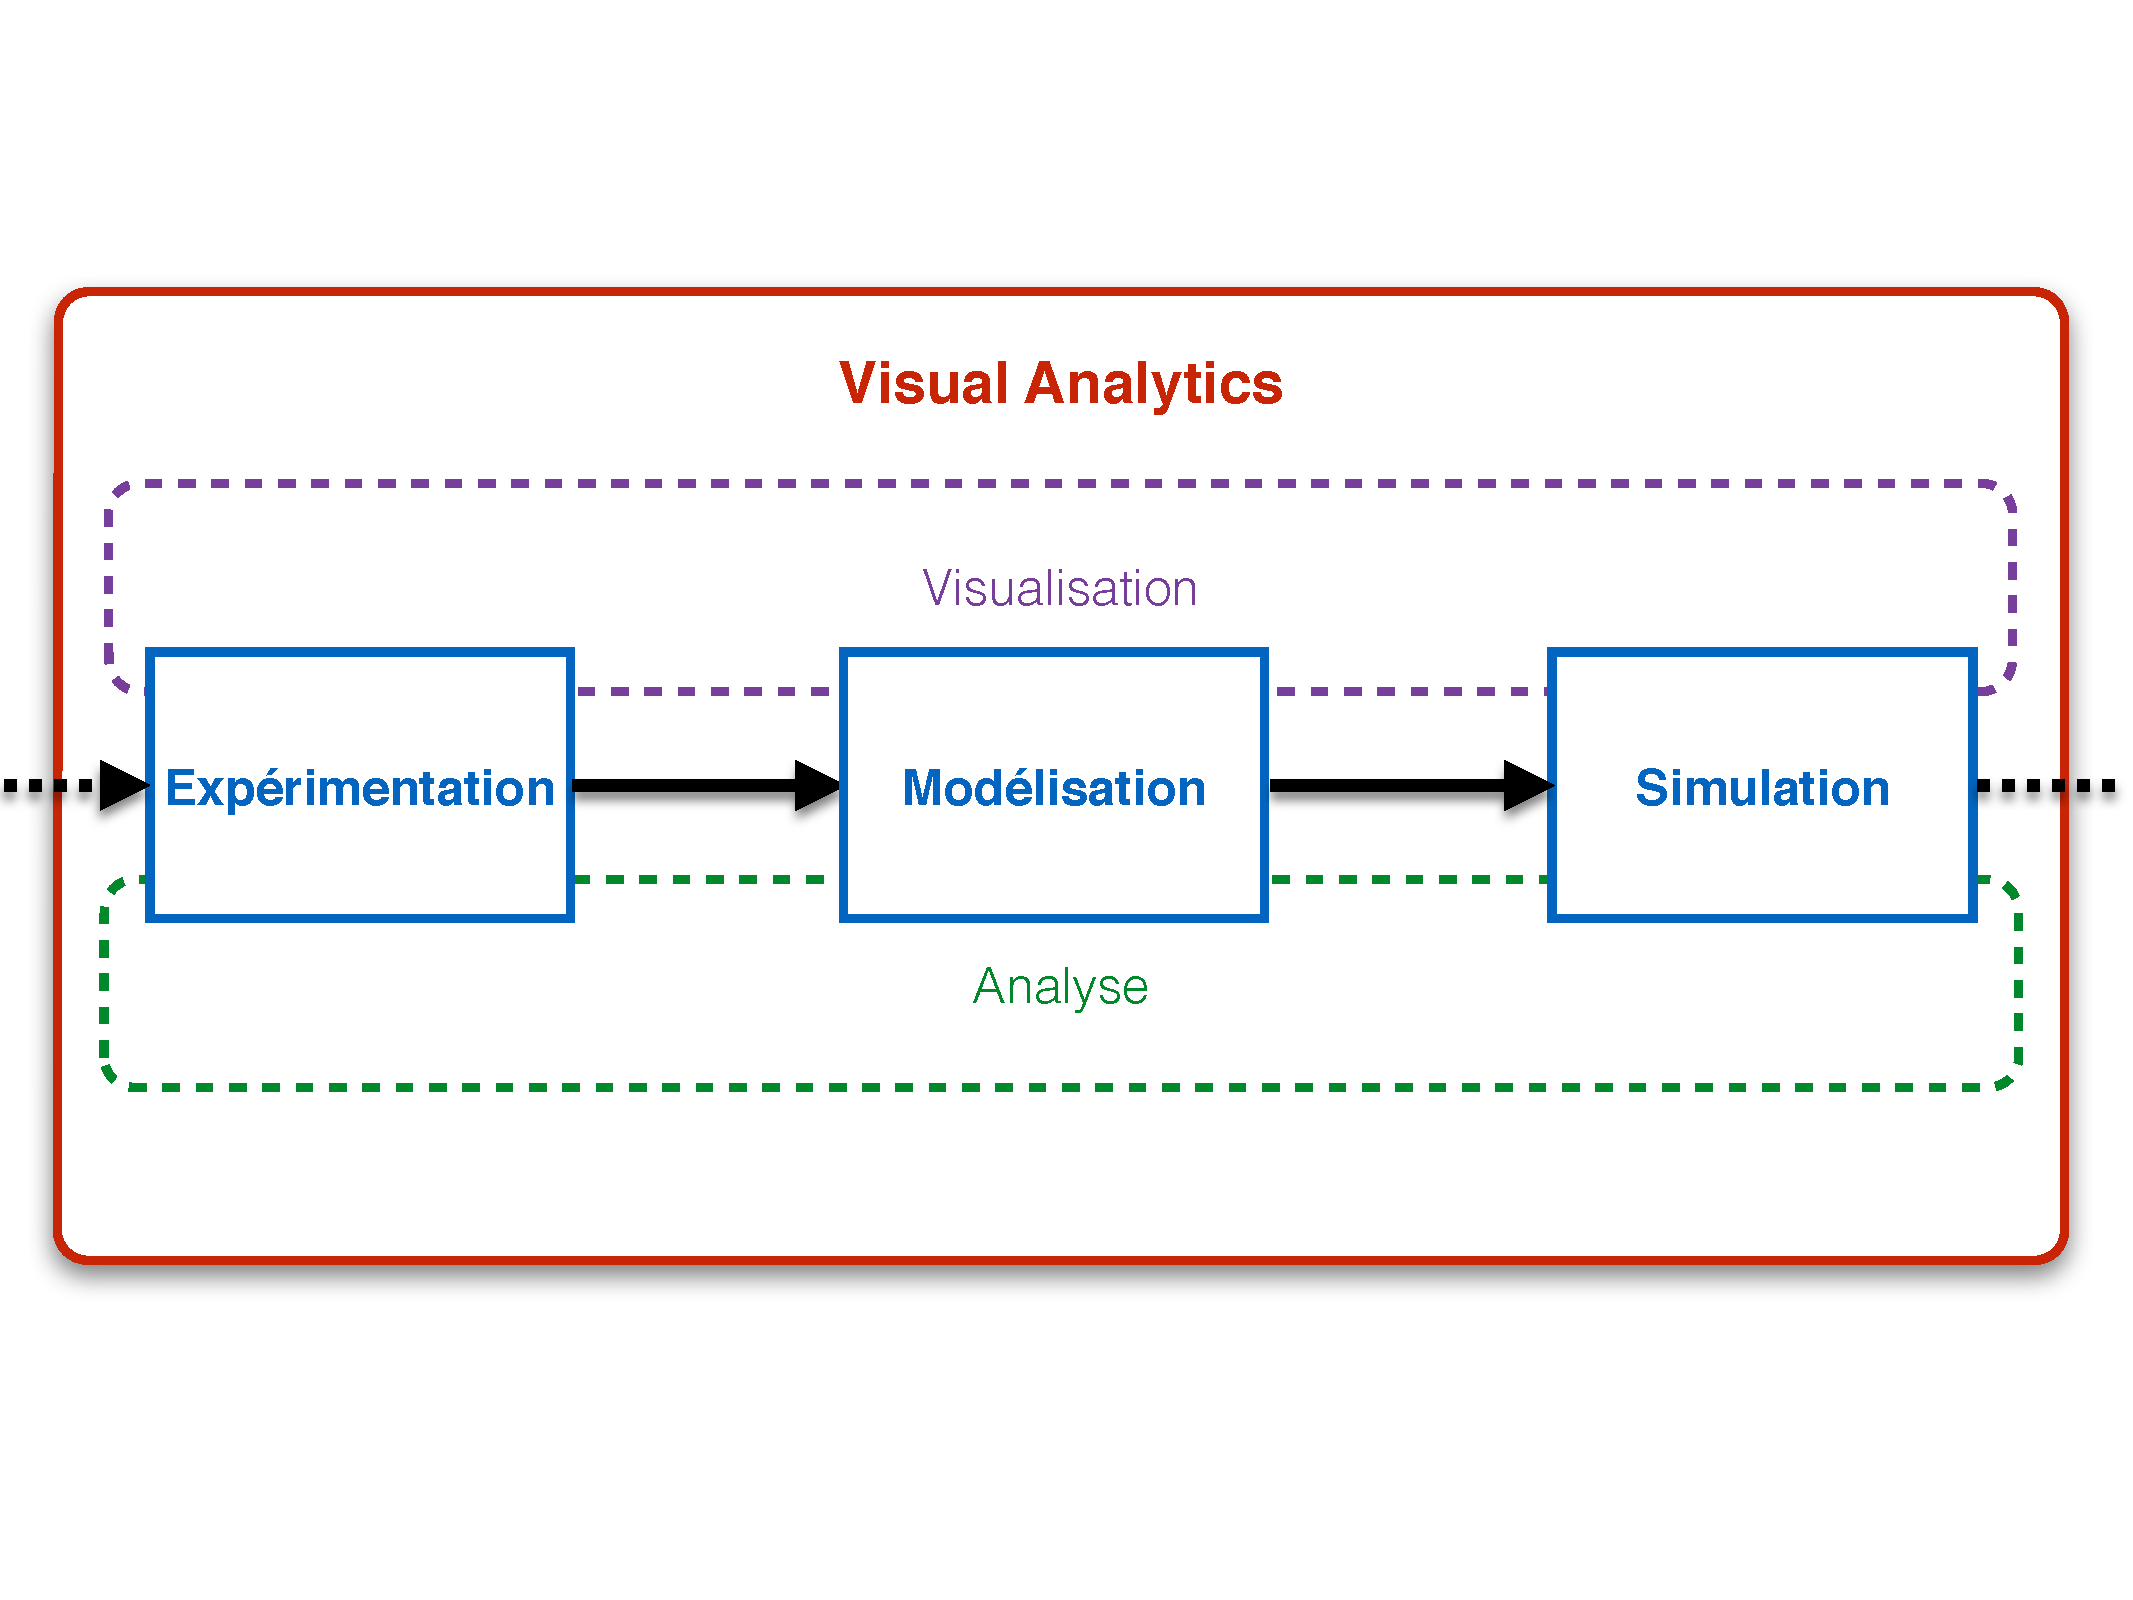
\includegraphics[width=1.0\linewidth]{./figures/ch5/process_bio_struct_VA}}
    \caption{\it Schéma du processus itératif d'étude d'une structure moléculaire en biologie structurale. Nous illustrons dans ce chapitre l'utilisation du Visual Analytics pour fusionner les outils de visualisation et d'analyse.}
  \label{Fig:process_bio_struct_VA}
  \hspace{0.3cm}
\end{figure}


\section{Approche applicative de la sémantique}

% Parmi les solutions possibles, une première pourrait être de mettre en place un suivi strict des données en assignant des identifiants uniques aux données représentant les mêmes concepts afin de garder une cohérence complète entre chaque élément affiché dans l'espace de visualisation et chaque élément de l'espace d'analyse. L'un des problèmes de cette solution se trouve dans la possibilité pour les espaces d'évoluer rapidement et demande donc ainsi une évolution constante du pool \commentaire{MB: pool en francais?} d'identifiants. 

% De plus, aucune information quant à la structure du complexe moléculaire ne serait extractible de ces identifiants, une gestion spécifique cherchant à maintenir la cohérence entre les identifiants du premier espace et les identifiants du second devrait ainsi être mise en place en parallèle.
% Une seconde solution est de donner au programme une couche d'abstraction supplémentaire via une définition ontologique des concepts manipulés afin de lui permettre de savoir quel concept est concerné par une éventuelle action (sélection, mise en avant, mise en arrière-plan, ...). 

% La définition ontologique des concepts manipulés, via une couche d'abstraction supplémentaire, permet à une application de savoir, à chaque action de l'utilisateur, 

Les outils du web sémantique décrits dans le chapitre précédent donnent une base de travail structurée pour intégrer des données liées au sein d'une plateforme. Cette plateforme n'est cependant pas déclinée et utilisée de la même façon pour l'ensemble des applications.

Factuellement, au sein du processus d'analyse structurelle et statistique d'une simulation dans un espace de travail fusionné, chaque élément avec lequel interagit l'utilisateur correspond à un individu unique dont la nature ou l'une de ses propriétés est mise en avant, soit à travers une représentation visuelle, soit à travers une représentation analytique. Chaque interaction avec cet individu devra déclencher un résultat dans tous les espaces possédant la référence d'au moins une de ses propriétés.

Cet objectif de fonctionnement implique que les concepts mis en jeu au sein de la plateforme doivent être correctement définis et aussi complets que possibles. La définition d'une sémantique pour ces concepts rempli ce rôle
En plus de lier étroitement les espaces partageant les représentations des mêmes individus, la représentation sémantique sous forme d'ontologie apporte différents avantages :

% doit permettre à l'utilisateur d'assimiler les concepts mis en jeu et donc d'avoir un contrôle possible sur sa base de faits (ou de données). Il sera en mesure d'ajouter des informations, de modifier

% , afin que l'utilisateur sache comment enrichir la base de données qui sera prise en entrée par les modules et afin que les données puissent être liées entre elles de façon optimale. La mise en place d'une ontologie permet que ces deux prérequis soient respectés. Le web sémantique tend à lier et structurer les données de façon à faciliter l'accès aux connaissances qu'elles contiennent. C'est également le but de notre étude et il semble adapté de reprendre les principes de cette approche afin de mettre en place la structure de notre base de données. Plusieurs avantages qu'offre la mise en place de données liées et d'une ontologie définissant les concepts étudiées peuvent être énumérés:

\begin{itemize}
    \item L'identification pour chaque interaction des concepts mis en jeu par l'utilisateur pour la proposition d'actions adaptées
    \item Représentation hiérarchisée des concepts obligeant une cohérence et une compatibilité des nouvelles connaissances/données
    \item Partage possible des données utilisées puisque estampillées autour d'un ensemble de définition précis
    \item Ontologie évolutive et potentiellement auto-extensible si des mécanismes d'interprétation des requêtes métier sont mis en place.
\end{itemize}

% Nous avons choisi comme support de représentation des données manipulées au sein de notre plateforme, la structure provenant du Web Sémantique basé sur le modèle RDF. L'avantage du langage RDF est sa possibilité d'être étendu et structuré grâce à une couche ontologique appelée \textit{Web Ontology Language} (OWL) qui reprend les critères standards des ontologies existantes et qui est le support de nombreuses ontologies recensées dans les portails officiels de bio-ontologies largement utilisées dans la communauté scientifique \cite{smith_obo_2007}. 

% \begin{figure}
%   \centering
%   {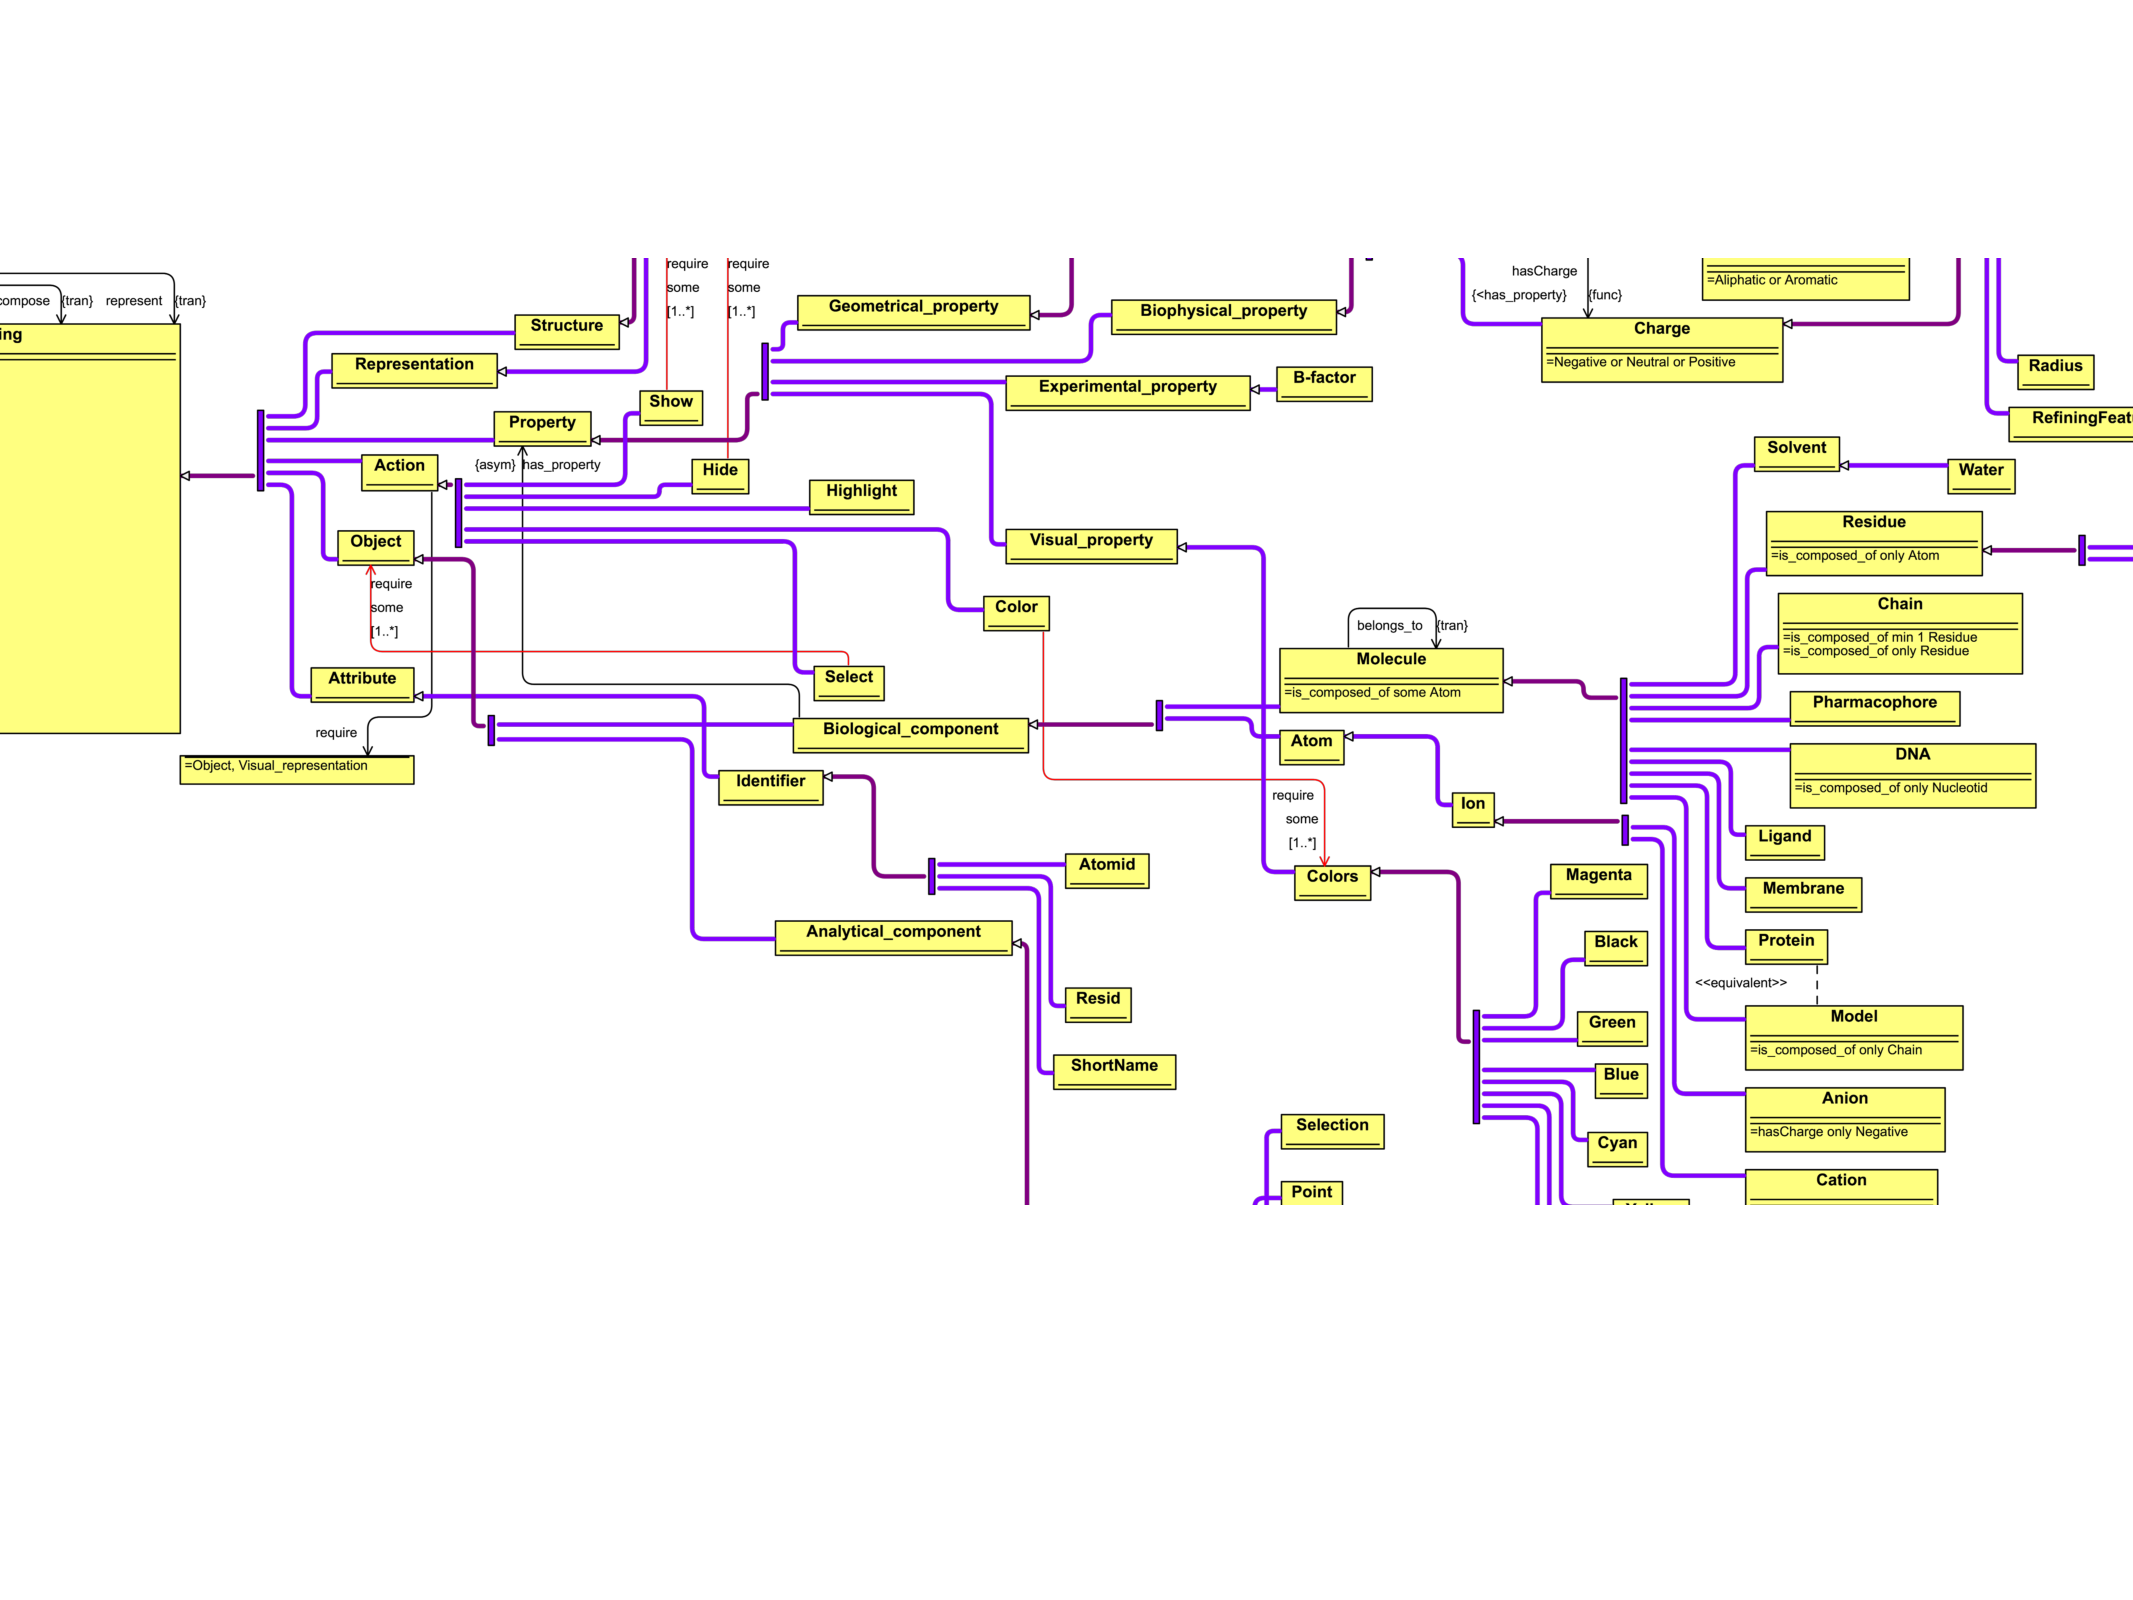
\includegraphics[width=.75\linewidth]{./figures/ch4/ch4_ontology.pdf}}
%     \caption{\it }
%   \label{Fig:extract_OWL_ontology}
%   \hspace{0.3cm}
% \end{figure}

\subsection{Ontologie OWL pour la modélisation des concepts de biologie structurale} \label{owl_ontology}

Comme le montre en partie la Figure \ref{Fig:ontology}, nous avons essayé de définir de façon complète l'ensemble des concepts que l'utilisateur aurait à manipuler lors de ses activités de visualisation et d'analyses synchronisées. 

Nous l'avons vu auparavant, plusieurs bio-ontologies ont été mises en place ces dernières années. Afin d'avoir une description la plus précise qui soit des concepts biologiques mis en jeu, nous nous sommes appuyés sur une ontologie déjà existante et disponible en ligne décrivant de façon complète les acides aminés et leurs propriétés \footnote{\url{http://bioportal.bioontology.org/ontologies/AMINO-ACID}}. Cette ontologie nous a permis de poser les bases biologiques d'un des principaux concepts de biologie structurale. En rassemblant des informations telles que la taille, l'hydrophobicité ou bien la charge de chaque acide-aminé il est ainsi possible d'extraire rapidement des groupes d'acides aminés possédant les mêmes propriétés et ainsi utiliser ces propriétés pour des raisonnements complexes lors de l'interrogation de la base de données. Parmi les nombreuses autres bio-ontologies disponibles, aucune d'entre-elles parvenait à définir aussi simplement que nous le désirions les autres concepts dont nous avions besoin. Il est cependant important de noter qu'une extension de notre ontologie est possible et même encouragée. Cette extension pourrait par exemple compléter et étoffer certaines propriétés biologiques omises mais intéressantes pour des études ponctuelles ou spécialisées.

L'ontologie a été conçue autour de 5 ensembles de définition distincts, s'adressant à 5 éléments différents composant notre plateforme : 

\begin{itemize}
  \item \textbf{Connaissance biologique} - Regroupe les concepts de biologie structurale et leurs propriétés
  \item \textbf{Représentation 3d} - Regroupe les moyens de représentation des modèles 3d
  \item \textbf{Représentation 2d} - Regroupe les moyens de représentation des analyses 2d
  \item \textbf{Interactions 3d} - Regroupe les modes et possibilités d'interaction dans l'espace de visualisation
  \item \textbf{Interactions 2d} - Regroupe les modes et possibilités d'interaction dans l'espace d'analyses
\end{itemize}

La distinction des ensembles de définition ne signifie pas que des liens existent entre ces ensembles, au contraire. La concept de <<Secondary Structure>> fait par exemple partie de l'ensemble de définition \textit{Connaissance biologique} mais est également rattaché au concept <<Cartoon>> de l'ensemble de définition \textit{Représentation 3d}. C'est l'ensemble de ces connections qui permettront par la suite de raisonner sur l'ontologie afin d'extraire des tâches automatisées au sein de moteurs de décision ou multimodaux.

Les concepts et propriétés présentes au sein des ensembles de définition de \textit{Représentation 2d} et de \textit{Représentation 3d} désignent les éléments graphiques permettant de représenter les concepts de l'ensemble des \textit{Connaissance biologique}. Les notions de forme, couleur mais également de types de graphes sont des notions qui seront définies dans ces ensembles. 
Il est à noter que les concepts analytiques sont définis par les éléments graphiques ou abstraits qui rentrent en jeu dans la création et la visualisation d'un résultat d'analyse, notions définies dans les deux ensemble de définition de \textit{Représentation}. Nous ne définissons cependant pas, volontairement, les processus d'analyse eux-mêmes car ceux-ci peuvent être de natures très différentes et possèdent un champ de définition bien trop large et complexe pour le sujet de cette thèse. Cela ne signifie pas que certains processus d'analyses ne seront pas utiliser au sein de la plateforme logicielle, il n'est simplement pas pertinent de les intégrer à l'ontologie, ne participant à l'uniformisation des rendus 3D et d'analyses.

En plus des concepts biologiques et de représentations cités précédemment, nous avons donc également cherché à définir tous les concepts d'interaction qui seront en jeu lors de la session d'utilisation de notre plateforme. Les interactions rassemblent toutes les actions que l'utilisateur pourrait vouloir effectuer sur les données qu'il manipule, de façon directe ou indirecte. Elles reprennent essentiellement les commandes permises par les logiciels de visualisation moléculaire et les outils d'analyse utilisés.

\begin{figure}
  \centering
  {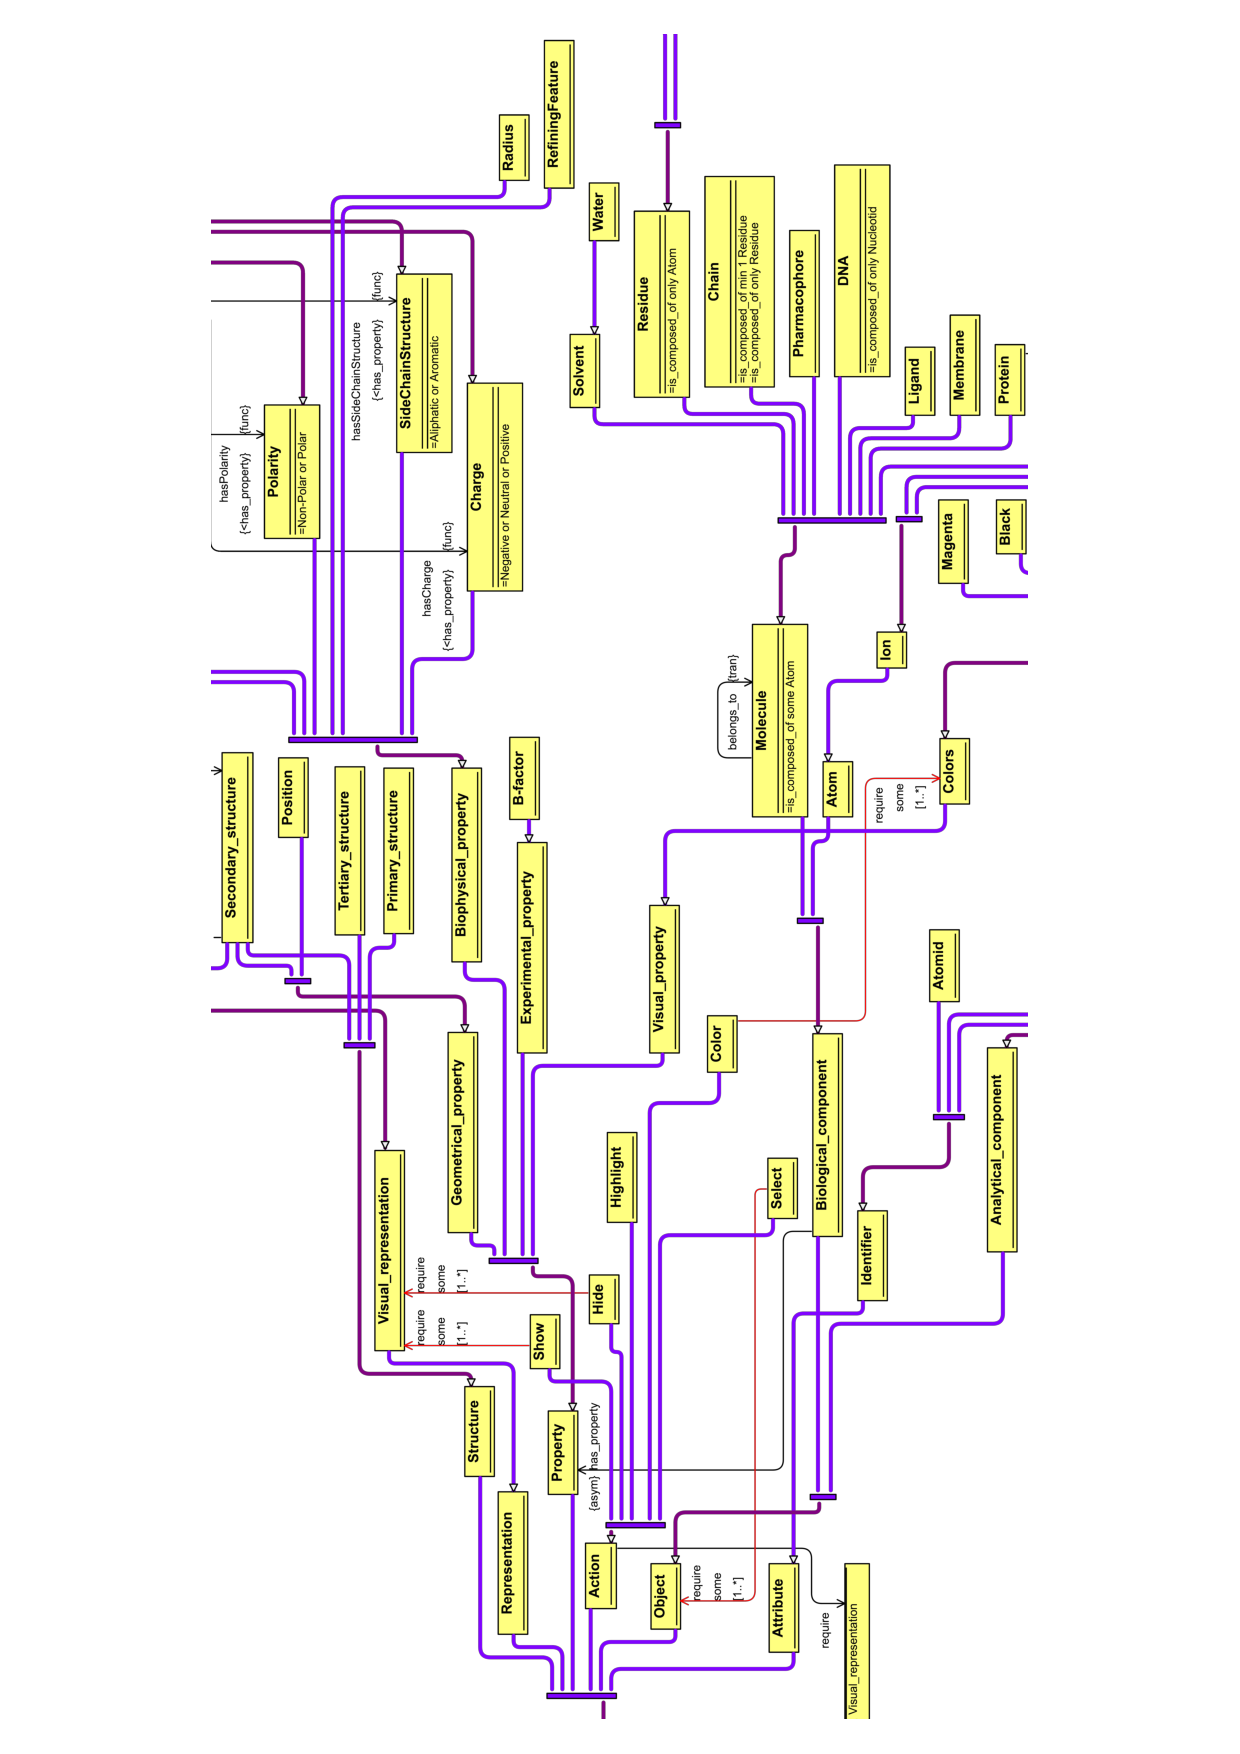
\includegraphics[width=0.8\linewidth]{./figures/ch5/ontology}}
    \caption{\it Extrait de l'ontologie OWL créée pour la mise en place de notre représentation sémantique de la plateforme logicielle. Visualisation obtenue avec OWLGrEd \cite{barzdins2010owlgred}}
  \label{Fig:ontology}
  \hspace{0.3cm}
\end{figure}

Une fois l'ontologie mise en place, il est possible d'alimenter la base de faits qu'elle définie en ajoutant les informations biologiques regroupées par l'expert scientifique. Ces informations vont devoir respecter le vocabulaire et la classification définie par les règles présentes dans l'ontologie OWL.

\subsection{Le RDF, format des bases de connaissances moléculaires} \label{rdf_import}

La description d'un environnement d'intérêt passe par l'analyse de toutes les informations biologiques pouvant être labellisées par une chaîne de caractère ou une valeur et qui correspondent à un concept ou une propriété identifiée dans l'ontologie OWL. Chaque information alimentera une base de données RDF organisant toutes les informations, de la même manière que pour les descriptions ontologiques, sous forme de triplets de type Sujet/Propriété/Objet.

Dans le cas qui nous intéresse pour ce travail de thèse, les simulations numériques moléculaires peuvent être découpées en une succession de modèles statiques 3D successifs. Chaque modèle correspond au concept \textit{Model} décrite dans notre ontologie. C'est le groupe structurel le plus large que nous ayons défini dans les composants structurels biologiques. Plusieurs triplets présents dans notre base de données finale sont illustrés dans le Listing \ref{rdf_xml}. Chaque atome présent dans un modèle possède une position 3d ainsi qu'un résidu auquel il appartient et indirectement, de la même manière, une chaîne et son modèle de référence grâce aux règles d'inférence. Ces informations n'ont pas besoin d'être spécifiées explicitement puisque les règles d'inférence définies dans l'ontologie instaurent, entre autres, le fait qu'un atome est sous-composant d'un résidu qui est un sous-composant d'une chaîne elle-même sous-composante d'un modèle. 
Cette information n'est donc pas présente dans la base de données sous forme d'un triplet explicite de type \textit{ATOM\_1234 my\:belongs\_to CHAIN\_12} mais ce triplet pourra être tout de même obtenu lors d'une requête cherchant à obtenir l'identifiant de la chaîne dont l'atome est l'un des composants. 

Toutes les propriétés géométriques (position, angles, distance, etc.), physico-chimiques (accessibilité, charge partielle, liaisons, etc.) ou analytiques (énergie, RMSD, température, etc.) pouvant être exportées des jeux de données étudiés sont donc intégrés dans la base de données de faits et surtout associés aux individus créés à partir des structures 3d de la simulation (atomes/résidus/chaîne/modèles). Ces individus sont des instances des concepts définis dans l'ontologie. Ils forment la population de la base de données et la majorité des propriétés définies se rapportent à eux.

Au-delà du stockage et de la mise à disposition des données suivant les règles pré-définies, la base de donnée RDF et plus particulièrement l'ontologie OWL la décrivant permettent de mettre en place des moteurs d'interprétation de commandes ou requêtes qui vont avoir pour objectif de récupérer une liste d'individus respectant un certain nombre de propriétés énoncées.

\begin{lstlisting}[language=XML, caption=Exemple de triplets RDF présents dans notre base de données, label=rdf_xml]

<owl:ObjectProperty rdf:about="&my;hasSize">
    <rdf:type rdf:resource="&owl;FunctionalProperty"/>
    <rdfs:domain rdf:resource="&my;AminoAcid"/>
    <rdfs:range rdf:resource="&my;Size"/>
    <rdfs:subPropertyOf rdf:resource="&my;has_property"/>
</owl:ObjectProperty>

<owl:DatatypeProperty rdf:about="&my;chain_id">
    <rdfs:range rdf:resource="&xsd;int"/>
</owl:DatatypeProperty>

<rdf:Description rdf:about="my:ATOM_36795">
	<my:atom_id rdf:datatype="http://www.w3.org/...#int">125</my:atom_id>
	<my:time_frame rdf:datatype="http://www.w3.org/...#int">190</my:time_frame>
	<rdf:type rdf:resource="my:Atom"/>
	<my:pos_z rdf:datatype="http://www.w3.org/...#double">22.33</my:pos_z>
	<my:atom_type>CB</my:atom_type>
	<my:pos_x rdf:datatype="http://www.w3.org/...#double">21.86</my:pos_x>
	<my:uniq_id rdf:datatype="http://www.w3.org/...#int">36795</my:uniq_id>
	<my:pos_y rdf:datatype="http://www.w3.org/...#double">31.6</my:pos_y>
	<my:belongs_to rdf:resource="my:RES_3622"/>
</rdf:Description>

\end{lstlisting}

\subsection{SPARQL, pour l'interaction directe} \label{sparql_interpretation_engine}

Lorsque les données ont été intégrées au sein de la base RDF, sous forme d'instance des concepts définis au sein de l'ontologie OWL, il est nécessaire de mettre en place un système d'interrogation et de récupération des données pour leur visualisation et traitement au sein de l'espace de travail de l'expert. Nous avons vu dans le chapitre précédent que RDF et OWL pouvaient être interrogés grâce au langage de requête SPARQL. A la manière du langage SQL pour les bases de données relationnelles, SPARQL est optimisé pour l'interrogation de bases RDF sous forme de triplets.

Notre implémentation de SPARQL a pris plusieurs formes afin de répondre à plusieurs besoins au sein de notre plateforme. Le premier besoin identifié et utilisé comme preuve de concept de notre structure ontologie OWL/base de données RDF fut la mise en place d'un moteur d'interprétation de mots-clés en commandes logicielles.

\subsection{Commande vocale : une approche par ensemble de mots-clés}

Une des techniques d'interaction plébiscitée au sein des environnements immersifs est la commande vocale. Elle traduit une phrase ou un groupe de mots édicté par l'utilisateur en une commande interprétable par la suite logicielle déclenchant ainsi une action appropriée. Les commandes vocales ont également pour intérêt de pouvoir être combinées à des commandes gestuelles. Un effet serait par exemple d'apporter un filtre supplémentaire sur le champ de sélection des objets virtuels concernés par une commande vocale.

Les actions identifiées au sein de notre programme impliquent pour une majorité d'entre elles une activité appliquée à un groupe structurel précis de l'ensemble moléculaire observé. Or ces groupes structurels peuvent être identifiés par des identifiants ayant un sens biologique (les acides aminés sont, de façon conventionnelle, numérotés séquentiellement au sein d'une chaîne de la partie N-terminale de la protéine vers la partie C-terminale), des identifiants uniques au sein de la base de données RDF ou bien leurs propriétés. Ainsi, pour interpréter les commandes émises en langage naturel par l'utilisateur, utilisant un vocabulaire spécifique du domaine avec un haut niveau d'abstraction, nous avons besoin d'une représentation qui peut porter la complexité des connaissances du domaine et relier les objets désignés par l'utilisateur aux objets virtuels d'intérêts.

Grâce à l'ontologie que nous avons mise en place, il est possible d'utiliser les capacités de raisonnement d'OWL ainsi que la puissance de SPARQL afin d'élaborer un moteur d'interprétation qui traduirait une commande vocale de l'utilisateur vers une commande spécifique appliquée de façon synchrone dans l'espace de visualisation et l'espace d'analyses.
Ce moteur peut être décomposé en 3 parties :

\begin{enumerate}
  \item Reconnaissance de mots-clés vocalisés par un logiciel dédié (\ref{Sphinx})
  \item Classification des mots-clés dans une structure décomposée de commande (\ref{classification_keywords})
  \item Construction de la commande finale opérationnelle (\ref{command})
\end{enumerate}

Nous détaillons ces 3 parties dans les sections ci-dessous.

\subsubsection{Reconnaissance de mots-clés métiers via Sphinx} \label{Sphinx}

La reconnaissance vocale en elle-même se fait via Sphinx. Ce logiciel de reconnaissance vocale base son processus de reconnaissance sur l'implémentation de dictionnaires créés auparavant et listant l'ensemble des termes pouvant être utilisés lors d'une session de travail. 
Ce dictionnaire se doit d'être le plus complet possible afin de prendre en compte l'ensemble du vocabulaire spécialisé que pourrait utiliser l'utilisateur. L'ontologie nous fournit justement une liste exhaustive des concepts manipulés au sein de la plateforme. Une liste complète des concepts et propriétés peut donc en être extraite afin de créer le dictionnaire métier sur lequel se basera Sphinx dans notre application.

Sphinx possède un module VRPN dédié nous permettant de l'intégrer aisément dans une architecture logicielle hiérarchisée. Sphinx analyse donc chaque commande vocale de l'utilisateur en la faisant correspondre au dictionnaire chargé afin d'en extraire les mots ou groupe de mots reconnus. Ces mots sont ensuite classés en groupes syntaxiques au sein dans une première partie du moteur d'interprétation que nous avons développé.

\subsubsection{Classification des mots-clés} \label{classification_keywords}

Une fois la réception des mots-clés effectuée, notre moteur va donc catégoriser chaque mot reçu. Cette classification se base sur le découpage de notre base de données qui différencie cinq catégories de mots pouvant être retrouvés dans une commande vocale :

\begin{itemize}
	\item \textbf{Action}
	\item \textbf{Composant}
	\item \textbf{Identifiant}
	\item \textbf{Propriété}
	\item \textbf{Représentation}
\end{itemize}

Cette classification est effectuée des requêtes SPARQL distinctes pour chaque catégorie et interrogeant l'ontologie OWL.

Alors que les catégories \textit{Action}, \textit{Composant}, \textit{Propriété} et \textit{Représentation} possèdent leurs propres concepts et peuvent être identifiées par un mot unique ($Hide$, $Chain$, $Charged$, $Sphere$, etc.), la catégorie \textit{Identifiant} est elle liée à une instance d'un concept de la catégorie \textit{Composant}. Étant donné la possible redondance des identifiants dans une base de donnée de simulation moléculaire puisque chaque modèle 3d décrit le même système moléculaire autant de fois qu'il y a d'unité de temps découpant la trajectoire, l'association entre un identifiant et un composant est obligatoire, quel que soit son niveau structurel. Un identifiant ne pourra donc être classé comme tel que si un composant existe, et seulement si ce composant possède effectivement l'identifiant demandé. Ce pré-requis constitue la première règle de notre classification de mots-clés.

Les commandes SPARQL permettant de dire si un mot-clé appartient ou non à une catégorie utilise l'opérateur \textit{ASK} qui prend en argument un ou plusieurs triplets et retourne un booléen \textit{true} si l'ensemble des triplets se vérifie (existe) dans la base de données. Les cinq requêtes SPARQL formulées pour la classification sont donc construites sur la même forme et illustrées dans le Listing \ref{sparql_cmd}. Les règles de raisonnement et d'inférence sont utilisées lors de l'ensemble des requêtes SPARQL. Par exemple, la requête

\begin{lstlisting}[language=XML]
ASK {my:Alanine rdfs:subClassOf my:Biological_component}
\end{lstlisting}

renverra donc \textit{true} malgré l'absence de lien direct, le concept \textit{Residue} se situant entre ces deux concepts (voir Figure \ref{alanine_owl}).

\begin{figure}
  \centering
  {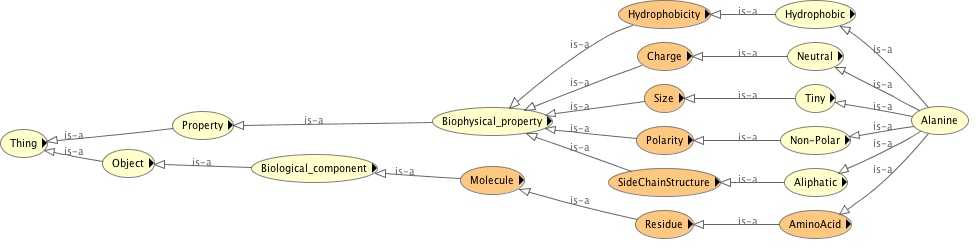
\includegraphics[width=0.8\linewidth]{./figures/ch5/alanine_owl}}
    \caption{\it Extrait de l'ontologie OWL créée pour la mise en place de notre représentation sémantique de la plateforme logicielle. Visualisation obtenue avec le plugin OWLViz de Protégé}
  \label{Fig:alanine_owl}
  \hspace{0.3cm}
\end{figure}

\begin{lstlisting}[language=XML, caption=\textit{Requêtes SPARQL effectuées pour tester la nature des mots-clés entrés par l'utilisateur}, label=sparql_cmd]
ASK {my:Hide rdfs:subClassOf my:Action}
ASK {my:Alanine rdfs:subClassOf my:Biological_component}
ASK {my:Cartoon rdfs:subClassOf my:Representation}
ASK {my:Red rdfs:subClassOf my:Colors}
ASK {my:Aliphatic rdfs:subClassOf my:Property}
\end{lstlisting}

\myparagraph{Action}

C'est le concept le plus simple à identifier parmi les mots-clés car il ne nécessite aucune association avec d'autres mots-clés dans notre représentation ontologique. Une liste précise d'actions a été identifiée et une correspondance simple nous permet de savoir si le mot employé est une action ou non.

\myparagraph{Composant}

Un composant est un ensemble d'atomes ou un unique atome identifié dans notre ontologie, soit par son niveau hiérarchique (modèle, chaîne, résidu, atome), soit par sa désignation directe (carbone, alanine, eau). Lorsqu'un composant est identifié, on cherchera toujours l'éventuelle présence d'un ou de plusieurs identifiants associés au sein de la liste de mots-clés extraite de la commande vocale.

\myparagraph{Identifiant}

Un identifiant ne peut être trouvé seul, il est toujours associé à un composant qu'il désigne. Les identifiants ont aussi la particularité de ne pas être recherché à un niveau ontologique mais au niveau de la base de données RDF puisqu'il n'existe pas de listes d'identifiants fixes dans notre ontologie, ces derniers variant entre les systèmes moléculaires étudiés. Lorsqu'un couple composant/identifiant existe au sein de la base de données, ces deux éléments sont regroupés et constituent un groupe syntaxique indépendant.

\myparagraph{Propriété}

Une propriété met en avant la particularité chimique, physique, biologique ou géométrique d'un composant. Les propriétés, à la différence des identifiants, constituent une liste finie dans notre ontologie et n'ont donc pas besoin d'être associé à un composant afin d'être identifiées. Cependant, certaines propriétés sont directement associées à un niveau hiérarchique précis au sein d'une protéine. On parlera par exemple d'un résidu hydrophobe mais jamais d'une chaîne hydrophile. La cohérence d'une propriété avec les concepts \textit{Composant} identifiés dans la commande doit donc être vérifiée. 

Les propriétés vont agir comme un filtre direct sur le sous-ensemble structurel sur lequel l'utilisateur veut agir. Ce filtre agira soit en unique sélecteur, rassemblant tous les individus appartenant à un groupe hiérarchique possédant la propriété identifiée, soit en filtre supplémentaire d'un sous-ensemble structurel ayant été identifié en parallèle grâce à d'autres concepts \textit{Composant}.

\myparagraph{Représentation}

Une représentation est une propriété visuelle associée directement et presque exclusivement à l'espace de visualisation. Les mots-clés désignant des concepts \textit{Représentation} sont associés aux actions centrées sur les changements de visualisation. Ils décrivent les états visuels sur lesquels l'utilisateur voudrait intervenir. Ils rassemblent par exemple les méthodes de représentation utilisés dans le visualiseur moléculaire, les couleurs utilisées, etc.
\\
\\
Une fois que chaque mot-clé est validé, c'est à dire identifié comme un concept (ou un individu pour les identifiants) et éventuellement associé à un autre mot-clé, il constitue un groupe syntaxique. Chaque groupe syntaxique possède une information qui correspond à différentes partie de la commande métier. Chaque type de commande est construite autour d'un agencement précis de groupes syntaxiques. On remarque que l'étape de classification possède une forte tolérance à l'ordre des mots-clés, ceux-ci pouvant être introduits dans n'importe quel ordre.


\subsubsection{De la commande vocale par mots-clés à la commande applicative} \label{command}

Au sein de notre programme, une commande vocale est composée d'une succession de groupements syntaxiques distincts mais liés les uns aux autres pour former une requête d'action. C'est l'unique type de commande présent pour le moment au sein de notre plateforme mais ses différentes déclinaisons permettent d'appliquer un large choix d'actions différentes sur les espaces de visualisation et d'analyses. Il est possible de décrire le type de commande que nous avons défini de la façon suivante :

$$action\ [paramètre]^+,\ (\ groupe\_structurel\ [identifiant]^+\ )^+$$

Les groupes syntaxiques sans crochets $[]$ sont obligatoires à l'inverse de ceux entre crochets qui sont optionnels. Le $^+$ désigne la possibilité d'avoir 0, 1 ou plusieurs occurrences du groupe syntaxique. Enfin les parenthèses désignent un bloc de groupes syntaxiques.

Cette représentation mathématique des groupes syntaxiques est présente dans notre ontologie. En effet, le concept \textit{Action} comporte dans sa définition ontologique un certain nombre de concepts associés, sous forme de pré-requis, nécessaires à son exécution. Ces pré-requis sont indispensables car ils se comportent comme des paramètres de la commande exécutée. Une action de type \textit{Color} nécessite par exemple la présence d'une propriété de type \textit{Colors} et d'une suite de mots-clés désignant un sous-ensemble structurel. 

De la même façon que pour l'action, la désignation d'un sous-ensemble structurel est obligatoire et peut être obtenu de différentes manières, dépendant directement du critère choisi par l'utilisateur pour filtrer les données sur lesquelles il souhaite appliquer son action. Les différentes manières d'obtenir un sous-ensemble structurel sont :

\begin{enumerate}
  \item Composant seul, l'ensemble des individus appartenant au concept indiqué sera pris en compte.
  \item Combinaison d'un composant moléculaire et d'un ensemble d'identifiant (unique, listé ou sous forme de plages continues). Cohérence entre identifiant et composant requis.
  \item Propriété seule, l'ensemble des individus possédant la propriété indiquée sera pris en compte.
  \item Combinaison d'un composant et d'une propriété. Cohérence nécessaire entre propriété et composant requis.
\end{enumerate}

Par soucis d'homogénéité, chaque sous-groupe structurel, mais s'il est désigné par un concept sans identifiant, est ramené à la liste d'individus le composant. SPARQL permet de récupérer directement les individus désignés par le sous-groupe structurel. Cette étape permet de désambiguïsé les résultats entre les commandes. La commande générée sera par contre plus complexe puisqu'elle comportera à chaque fois la liste détaillée des individus concernés par la commande.

Par défaut, le sous-ensemble structurel désigné dans la commande vocale dépendra directement du jeu de données affiché dans l'espace de travail afin d'éviter une surcharge de précision à donner par l'utilisateur. Par exemple, si deux modèles sont affichés dans l'espace de travail, la commande \textit{Alanine 147} désignera uniquement les alanines dont l'identifiant est 147 parmi les deux modèles affichés.

Si tous les pré-requis associés à une action sont respectés, alors la commande est ordonnée de façon à respecter la syntaxe de l'environnement de visualisation utilisé. La dernière étape est donc une simple transformation des concepts et des individus en une formulation compréhensible par les espaces de travail.

\subsubsection{Performance}




\begin{figure}
  \centering
  {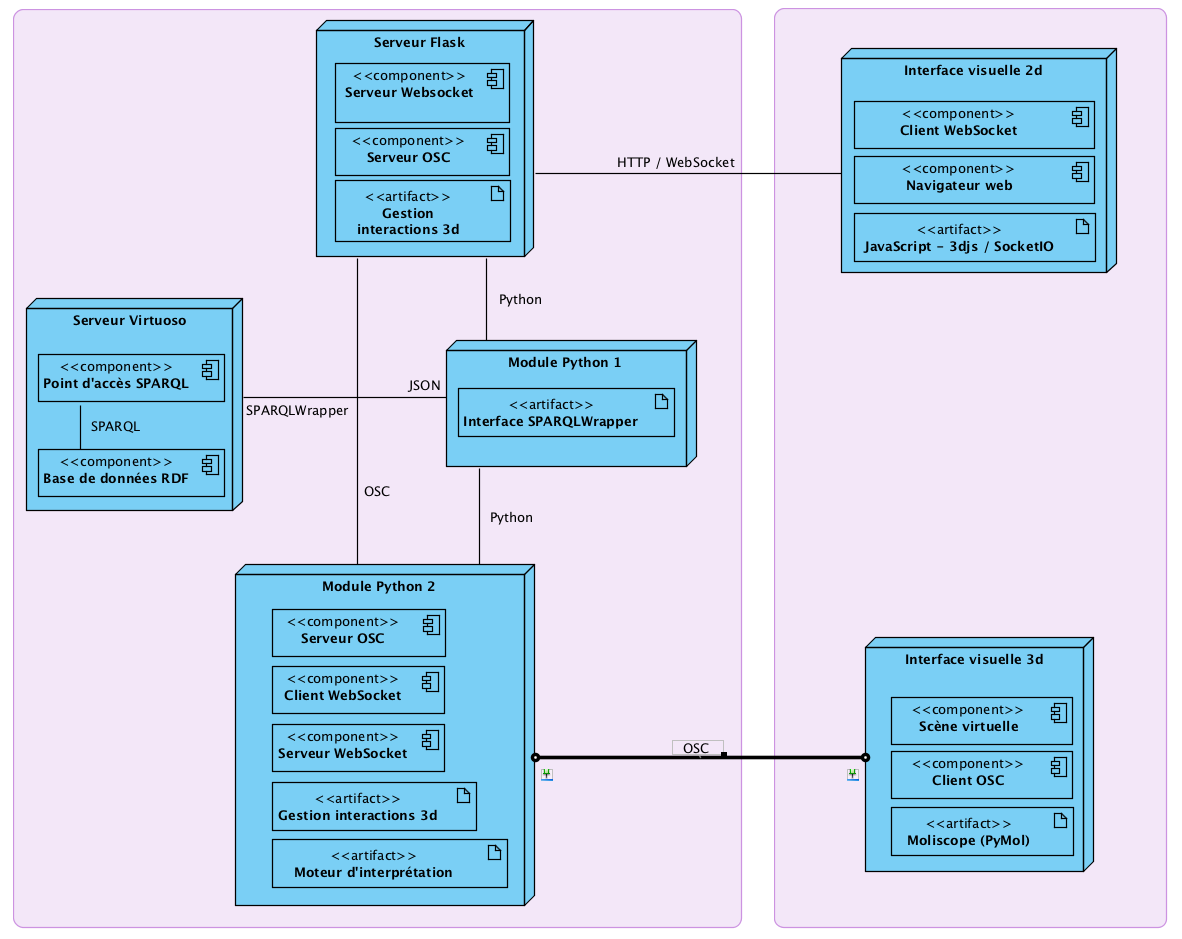
\includegraphics[width=.75\linewidth]{./figures/ch5/platform_architecture}}
    \caption{{\it Diagramme de déploiement des modules et leur connectivité au sein de notre plateforme immersive de Visual Analytics.}}
  \label{Fig:platform_architecture}
  \hspace{0.3cm}
\end{figure}


\section{Vers une approche de Visual Analytics immersive pour la biologie structurale}

L'ontologie métier définie dans la section \ref{owl_ontology} et la base de données générée à partir de données de simulation moléculaire dans la section \ref{rdf_import} nous ont permis de mettre en place un espace de travail combinant visualisation et analyses reposant repose exclusivement sur une interrogation constante de la base de données grâce à SPARQL.

La conception de notre programme repose sur une architecture logicielle complexe. Dans le schéma illustré dans la Figure \ref{Fig:schema_prog_visu_ana}, nous l'avons volontairement placé au centre d'une boucle bi-latérale de communication reliant l'espace de visualisation à l'espace d'analyse.

Notre base de données est hébergée dans un serveur web Virtuoso accessible depuis le réseau afin de garantir un accès privilégié et optimisé à nos données. 

Notre cas d'étude est une simulation moléculaire test reprenant l'évolution structurelle et énergétique d'une protéine transmembranaire, GLIC, pendant 2 ns ($2*10^{-9}$s). Des modèles statiques de cette évolution ont été générés tous les 8 ps ($2*10^{-12}$s) créant ainsi 251 fichiers PDB. Le système contient également un ligand identifié de GLIC, le bromoforme, dont on cherche à connaître le mode de liaison et surtout son impact sur la forme de GLIC au cours du temps. Le solvant utilisé pour la simulation est un modèle simplifié <<gros-grain>> d'eau.

\subsection{Création de la base de donnée RDF}

Comme nous l'avons évoqué précédemment, nous avons mis en place une ontologie OWL regroupant l'ensemble des concepts que les experts seraient amenés à manipuler ou visualiser durant leur travail au sein de notre programme. Cette ontologie a été créée grâce à Protégé \footnote{\url{http://protege.stanford.edu/}}, une structure logicielle et éditeur d'ontologies regroupant plusieurs outils pour la création, l'édition et l'interrogation d'ontologies OWL.

\begin{figure}
  \centering
  {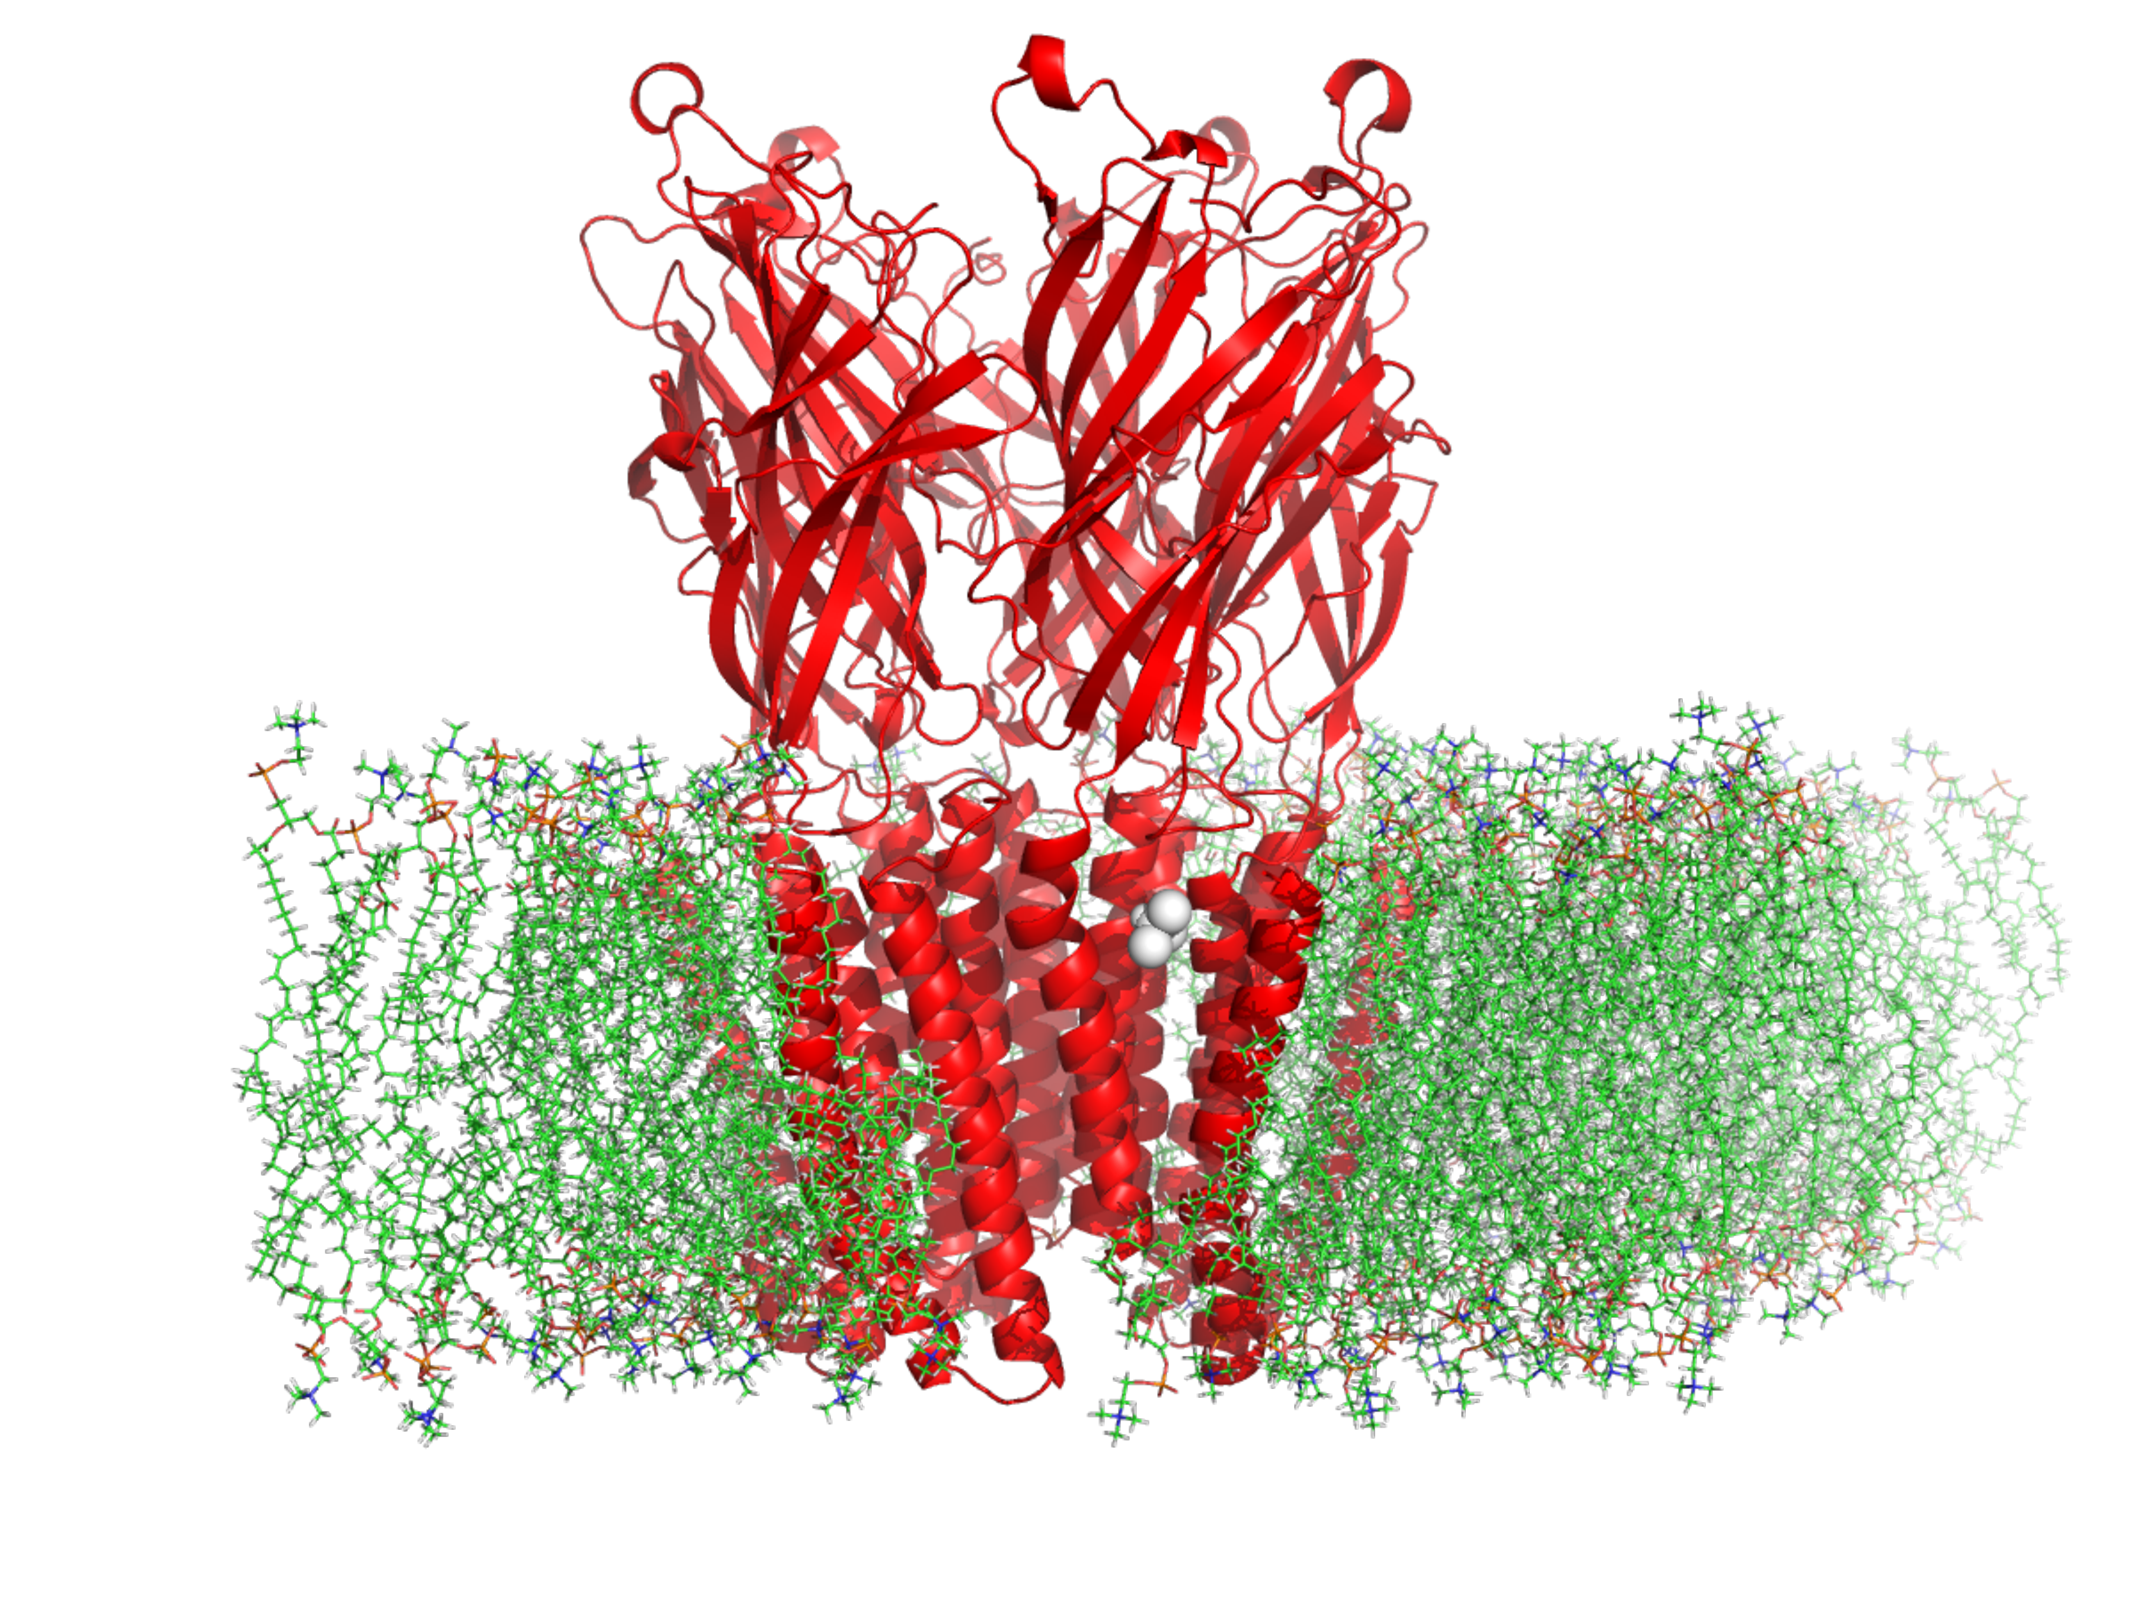
\includegraphics[width=.75\linewidth]{./figures/ch5/glic+bromoform.pdf}}
    \caption{{\it Rendu graphique de la liaison d'un bromoforme (sphères blanches) sur la protéine GLIC (<<cartoon>> rouge) au sein d'une membrane cellulaire (lignes vert).}}
  \label{Fig:glic+bromoform}
  \hspace{0.3cm}
\end{figure}

Concernant la partie expérimentale, nous sommes partis de données réelles de simulation moléculaires générées par des experts du domaine. La trajectoire étudiée correspond à une dynamique moléculaire d'une protéine transmembranaire, GLIC, et d'un ligand connu pour être un de ses inhibiteurs, le bromoforme. Cette simulation de 2 nanosecondes a été effectué en solvant explicite grâce à un modèle d'eau standard, XXX et met en évidence la présence du bromoforme dans plusieurs sites de liaisons de la protéine. GLIC est une protéine responsable de la perméation de la cellule puisqu'elle régule le passage des molécules d'eau et des ions entre la partie extra- et intra-cellulaire des cellules. Plusieurs anesthésiques ont été identifié comme possédant une affinité suffisante avec GLIC pour qu'une liaison s'effectue, le bromoforme étant un des ligands concernés. La structure générale de GLIC ainsi que du bromoforme peut être observée dans la Figure \ref{Fig:glic+bromoform}. Le choix de GLIC ne fut pas anodin, trois grandes raisons ont dictées notre décision :
\begin{enumerate}
	\item C'est une protéine bien connue des experts avec lesquels nous travaillons, il est ainsi aisé d'identifié les analyses pertinentes que nous pourrons associées par la suite.
	\item La taille de GLIC est relativement importante, en particulier lorsque la membrane est représentée, nous considérons donc ce complexe comme un cas d'étude intéressant pour tester les limites de nos méthodes en terme de performance.
	\item L'environnement de GLIC est très hétérogène, permettant de manipuler des concepts comme les membranes et les ligands et donc de vérifier la robustesse de notre programme pour des concepts particuliers.
\end{enumerate}

La transformation des données expérimentales en triplets RDF s'est faite grâce à Jena, une librairie Java permettant la manipulation de données RDF/OWL via le langage Java. Cette librairie permet de charger une ontologie sous différents formats, dont plusieurs supportés par Protégé lors de l'export, et de s'appuyer dessus afin de créer les individus correspondants aux concepts ontologiques définis. Chaque individu découle d'un ensemble de données obtenu à partir des fichiers caractérisant la simulation moléculaire étudiée. Dans notre cas, nous nous appuyons essentiellement sur des fichiers PDB décrivant la structure 3d des modèles à chaque pas de temps de la simulation. Ces fichiers possèdent les identifiants des différents groupes structurels qui seront manipulés (atomes/acides-aminés/chaînes), les coordonnées 3d des atomes ainsi que les liens des groupes structurels entre-eux. Des fichiers regroupant des données expérimentales telles que les énergies ou les températures ou bien des données analytiques comme les distances inter-atomes sont également utilisés en entrée de notre programme Java afin que leurs valeurs soient associés aux individus qu'ils décrivent. Les triplets créés dans Jena sont sauvegardées dans des fichiers texte sous différents formats : RDF/XML, N3 ou Turtle. Le processus est schématisé dans la Figure \ref{Fig:pdb_parsing_to_ttl}.


\begin{figure}
  \centering
  {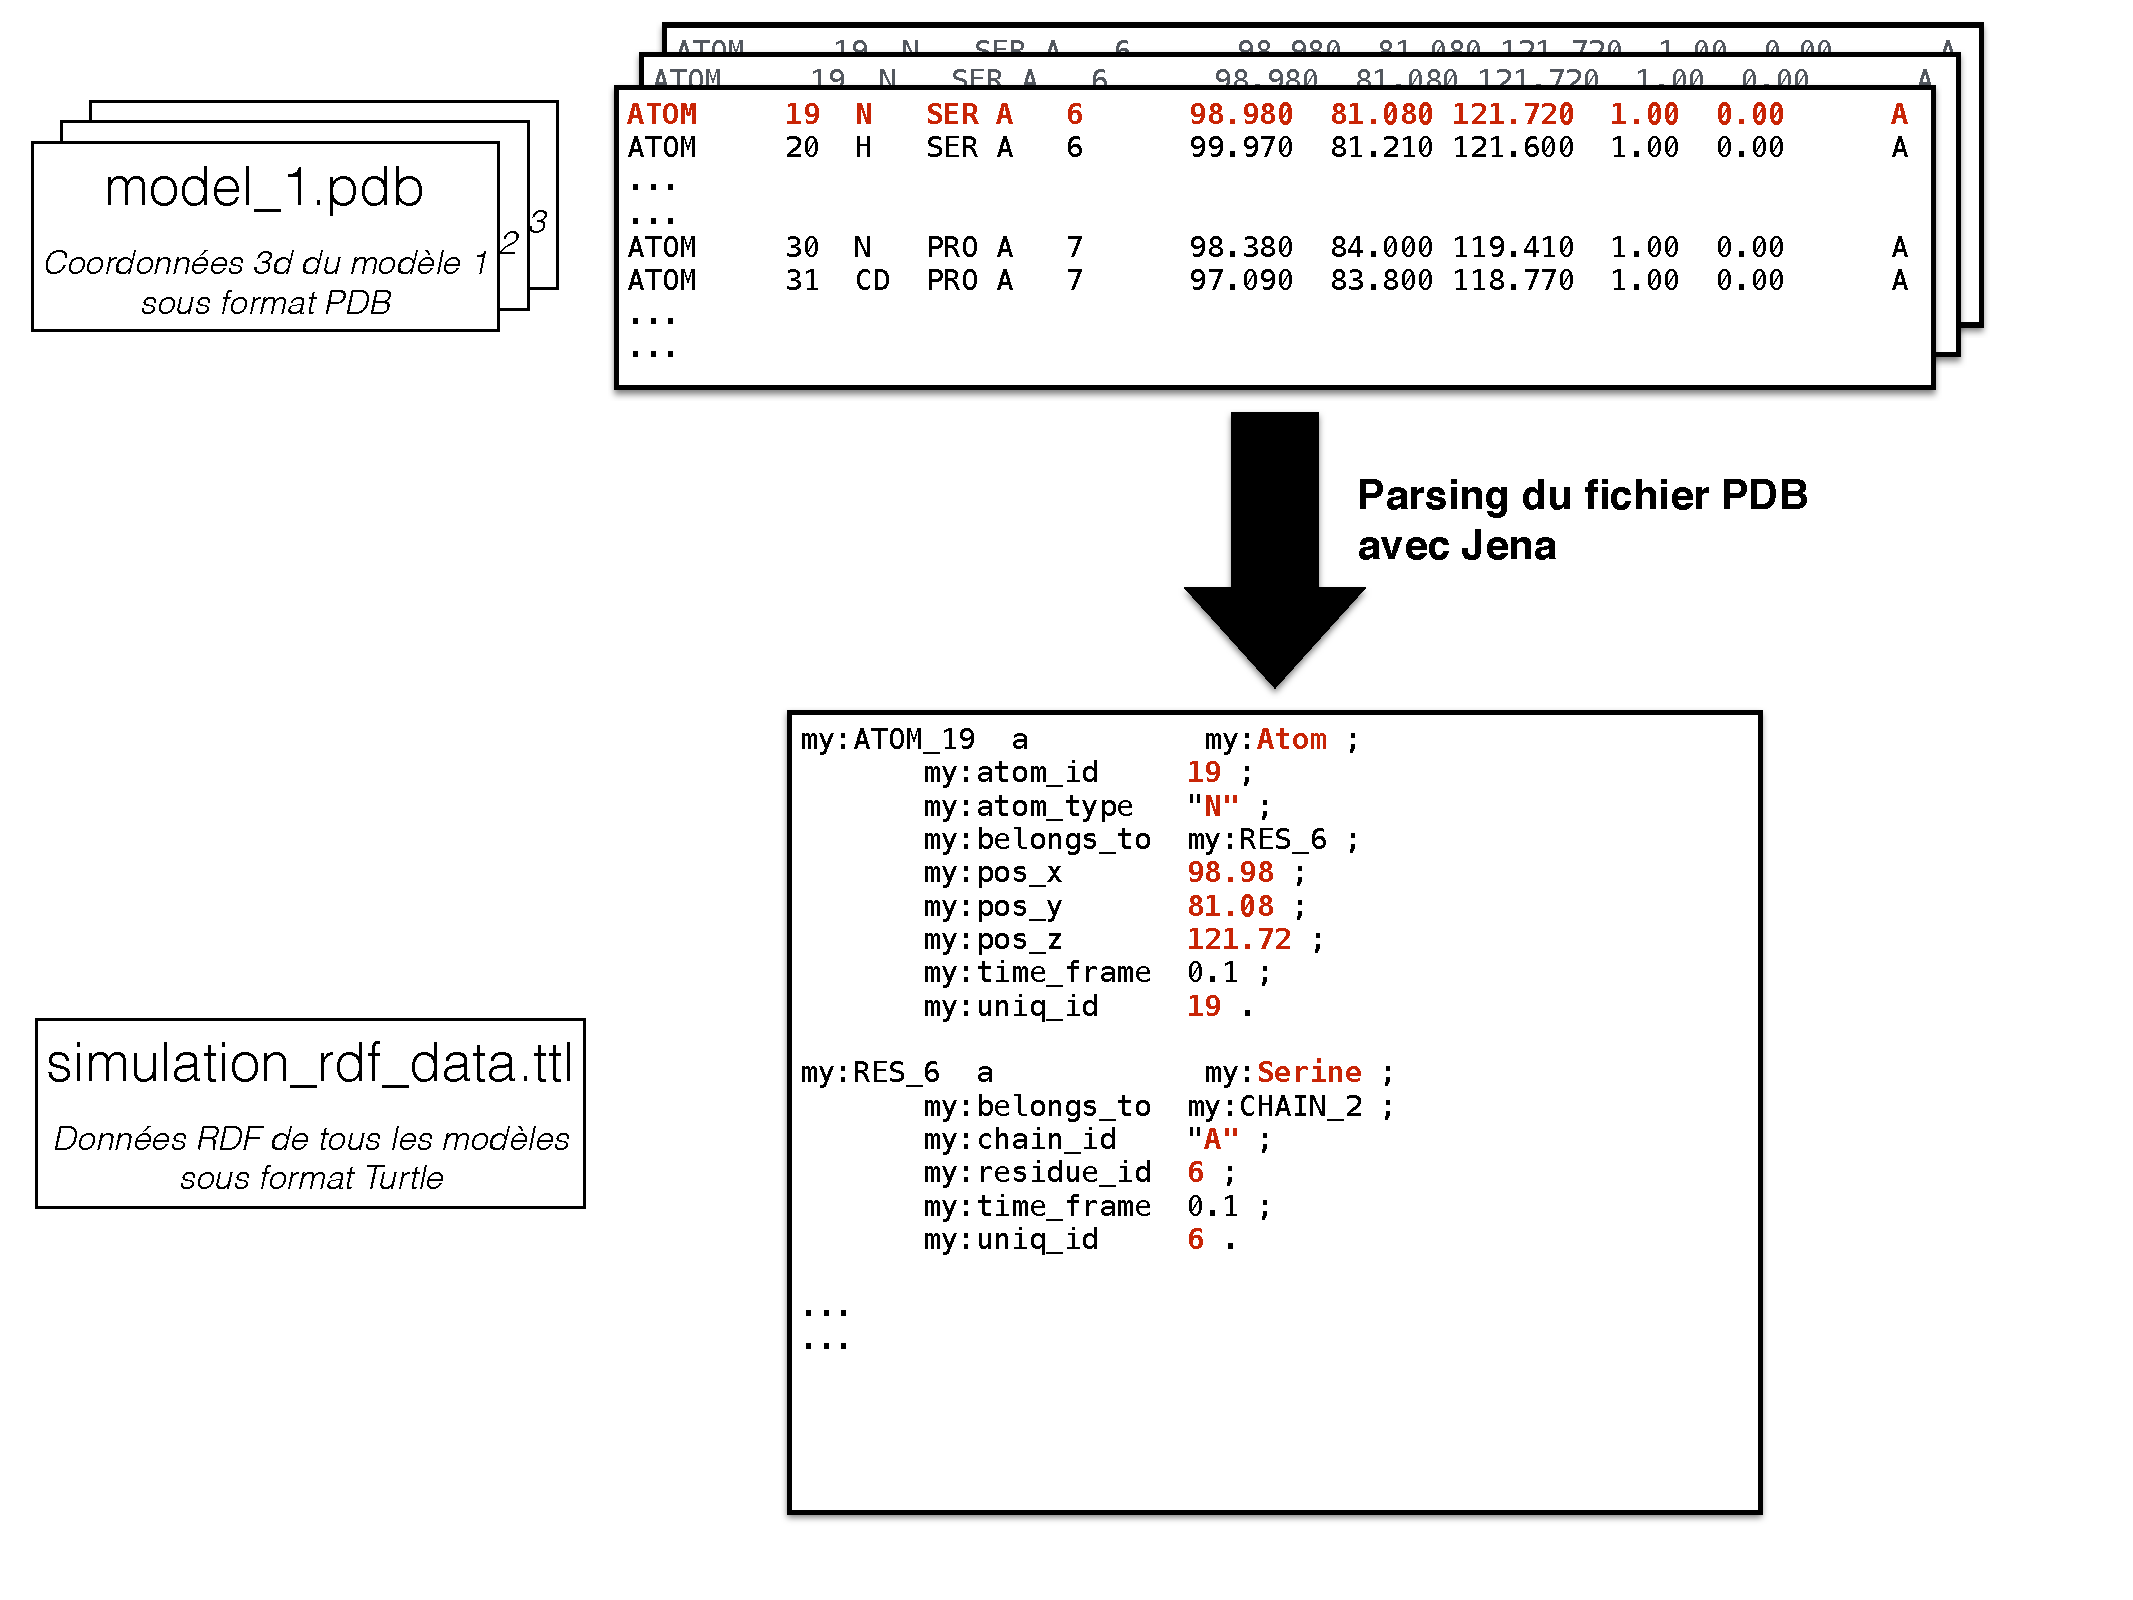
\includegraphics[width=.75\linewidth]{./figures/ch5/pdb_parsing_to_ttl.pdf}}
    \caption{{\it Schéma du processus de parsing effectué au sein d'un module Java utilisant la librairie de gestion de données OWL/RDF(S) Jena. Les fichiers PDB ont été obtenus à partir d'une simulation moléculaire et chaque PDB représente la conformation spatiale du système simulé à un instant $t$.}}
  \label{Fig:pdb_parsing_to_ttl}
  \hspace{0.3cm}
\end{figure}

L'ontologie est faite de telle sorte qu'il soit possible d'ajouter a posteriori des valeurs physico-chimiques ou d'analyses que l'utilisateur voudrait associer à la trajectoire étudiée. Il est par exemple possible d'effectuer une analyse d'accessibilité des atomes ou des acides-aminés à la suite de la simulation et de charger les résultats pour les individus déjà existants dans la base de données. Cette possibilité nous permettra également de mettre en place des modules <<optionnels>> d'analyses que l'utilisateur pourra utiliser pendant sa session de travail et qui viendront ajouter les résultats obtenus directement dans la base de données pour une visualisation de ceux-ci de façon complètement intégrée. En plus du gain de temps et d'uniformisation, cela permet de sauvegarder toutes nouvelles données générées lors de la session de travail et donc de les réutiliser par la suite sans besoin de relancer les modules d'analyses ayant servi à leur création.

Les fichiers générés, celui de l'ontologie et celui des triplets RDF, sont ensuite chargés au sein d'un serveur Virtuoso \footnote{\url{http://virtuoso.openlinksw.com/}} qui est un serveur de gestion de données dont l'architecture permet le stockage de données RDF de façon optimisée et met en place un point d'accès à ces données via un espace de requêtes SPARQL. Ce point d'accès se fait via une adresse URL que la plupart des librairies prenant en charge le SPARQL utilisent comme interface sur les données RDF. La version du serveur Virtuoso que nous utilisons permet la mise en place les règles d'inférence OWL-Lite pour chaque requête SPARQL effectuée, aspect très important pour notre plateforme.

\subsection{Gestion des données RDF et requêtes SPARQL}

Dans le but de mettre en place une interface entre les différents modules et la base de données RDF, nous avons mis en place un module spécifique contenant un ensemble de fonctions permettant de lancer des requêtes SPARQL sur la base de données. 
Cette interface sous forme de module Python utilise la librairie SPARQLWrapper \footnote{\url{https://rdflib.github.io/sparqlwrapper/}} qui permet d'accéder à tout point d'accès SPARQL via une URL, de lancer une requête et de récupérer les résultats sous format JSON, ensuite facilement convertissables en dictionnaires Python. Les résultats sont ensuite transmis aux modules ayant appelé une fonction de cette interface. Dans notre cas, le serveur Virtuoso hébergeant la base de données fournie le point d'accès SPARQL nécessaire et permet ainsi l'interfaçage du module avec la base de donnée RDF que nous avons créé (cf. Figure \ref{Fig:platform_architecture}).

\subsection{Visualisation des données moléculaire 3d}

Nous avons choisi PyMol \cite{delano_pymol_2002} comme programme de visualisation moléculaire 3d. PyMol est un logiciel de visualisation très utilisé dans la communauté scientifique et qui possède une API complète qui facilite son intégration au sein d'une plateforme logicielle basée sur des modules hétérogènes. 
Nous avons utilisé cette API pour automatiser plusieurs étapes du chargement des trajectoires de simulation. Au-delà du simple chargement visuel des structures 3d de molécules et de leur rendu, nous avons mis en place au sein de PyMol des processus spécifiques surveillant les actions de l'utilisateur dans l'espace de visualisation. 
Plusieurs actions, dont notamment celle de sélection, peuvent déclencher un événement qui se répercutera de façon synchrone avec l'espace d'analyse. Le portage de PyMol dans des environnements immersifs est un projet en cours sous le nom <<Moliscope>> et nous profitons des derniers développements de ce projet pour notre programme (voir Figure \ref{Fig:multi_collaboratif}).

\begin{figure}
  \centering
  {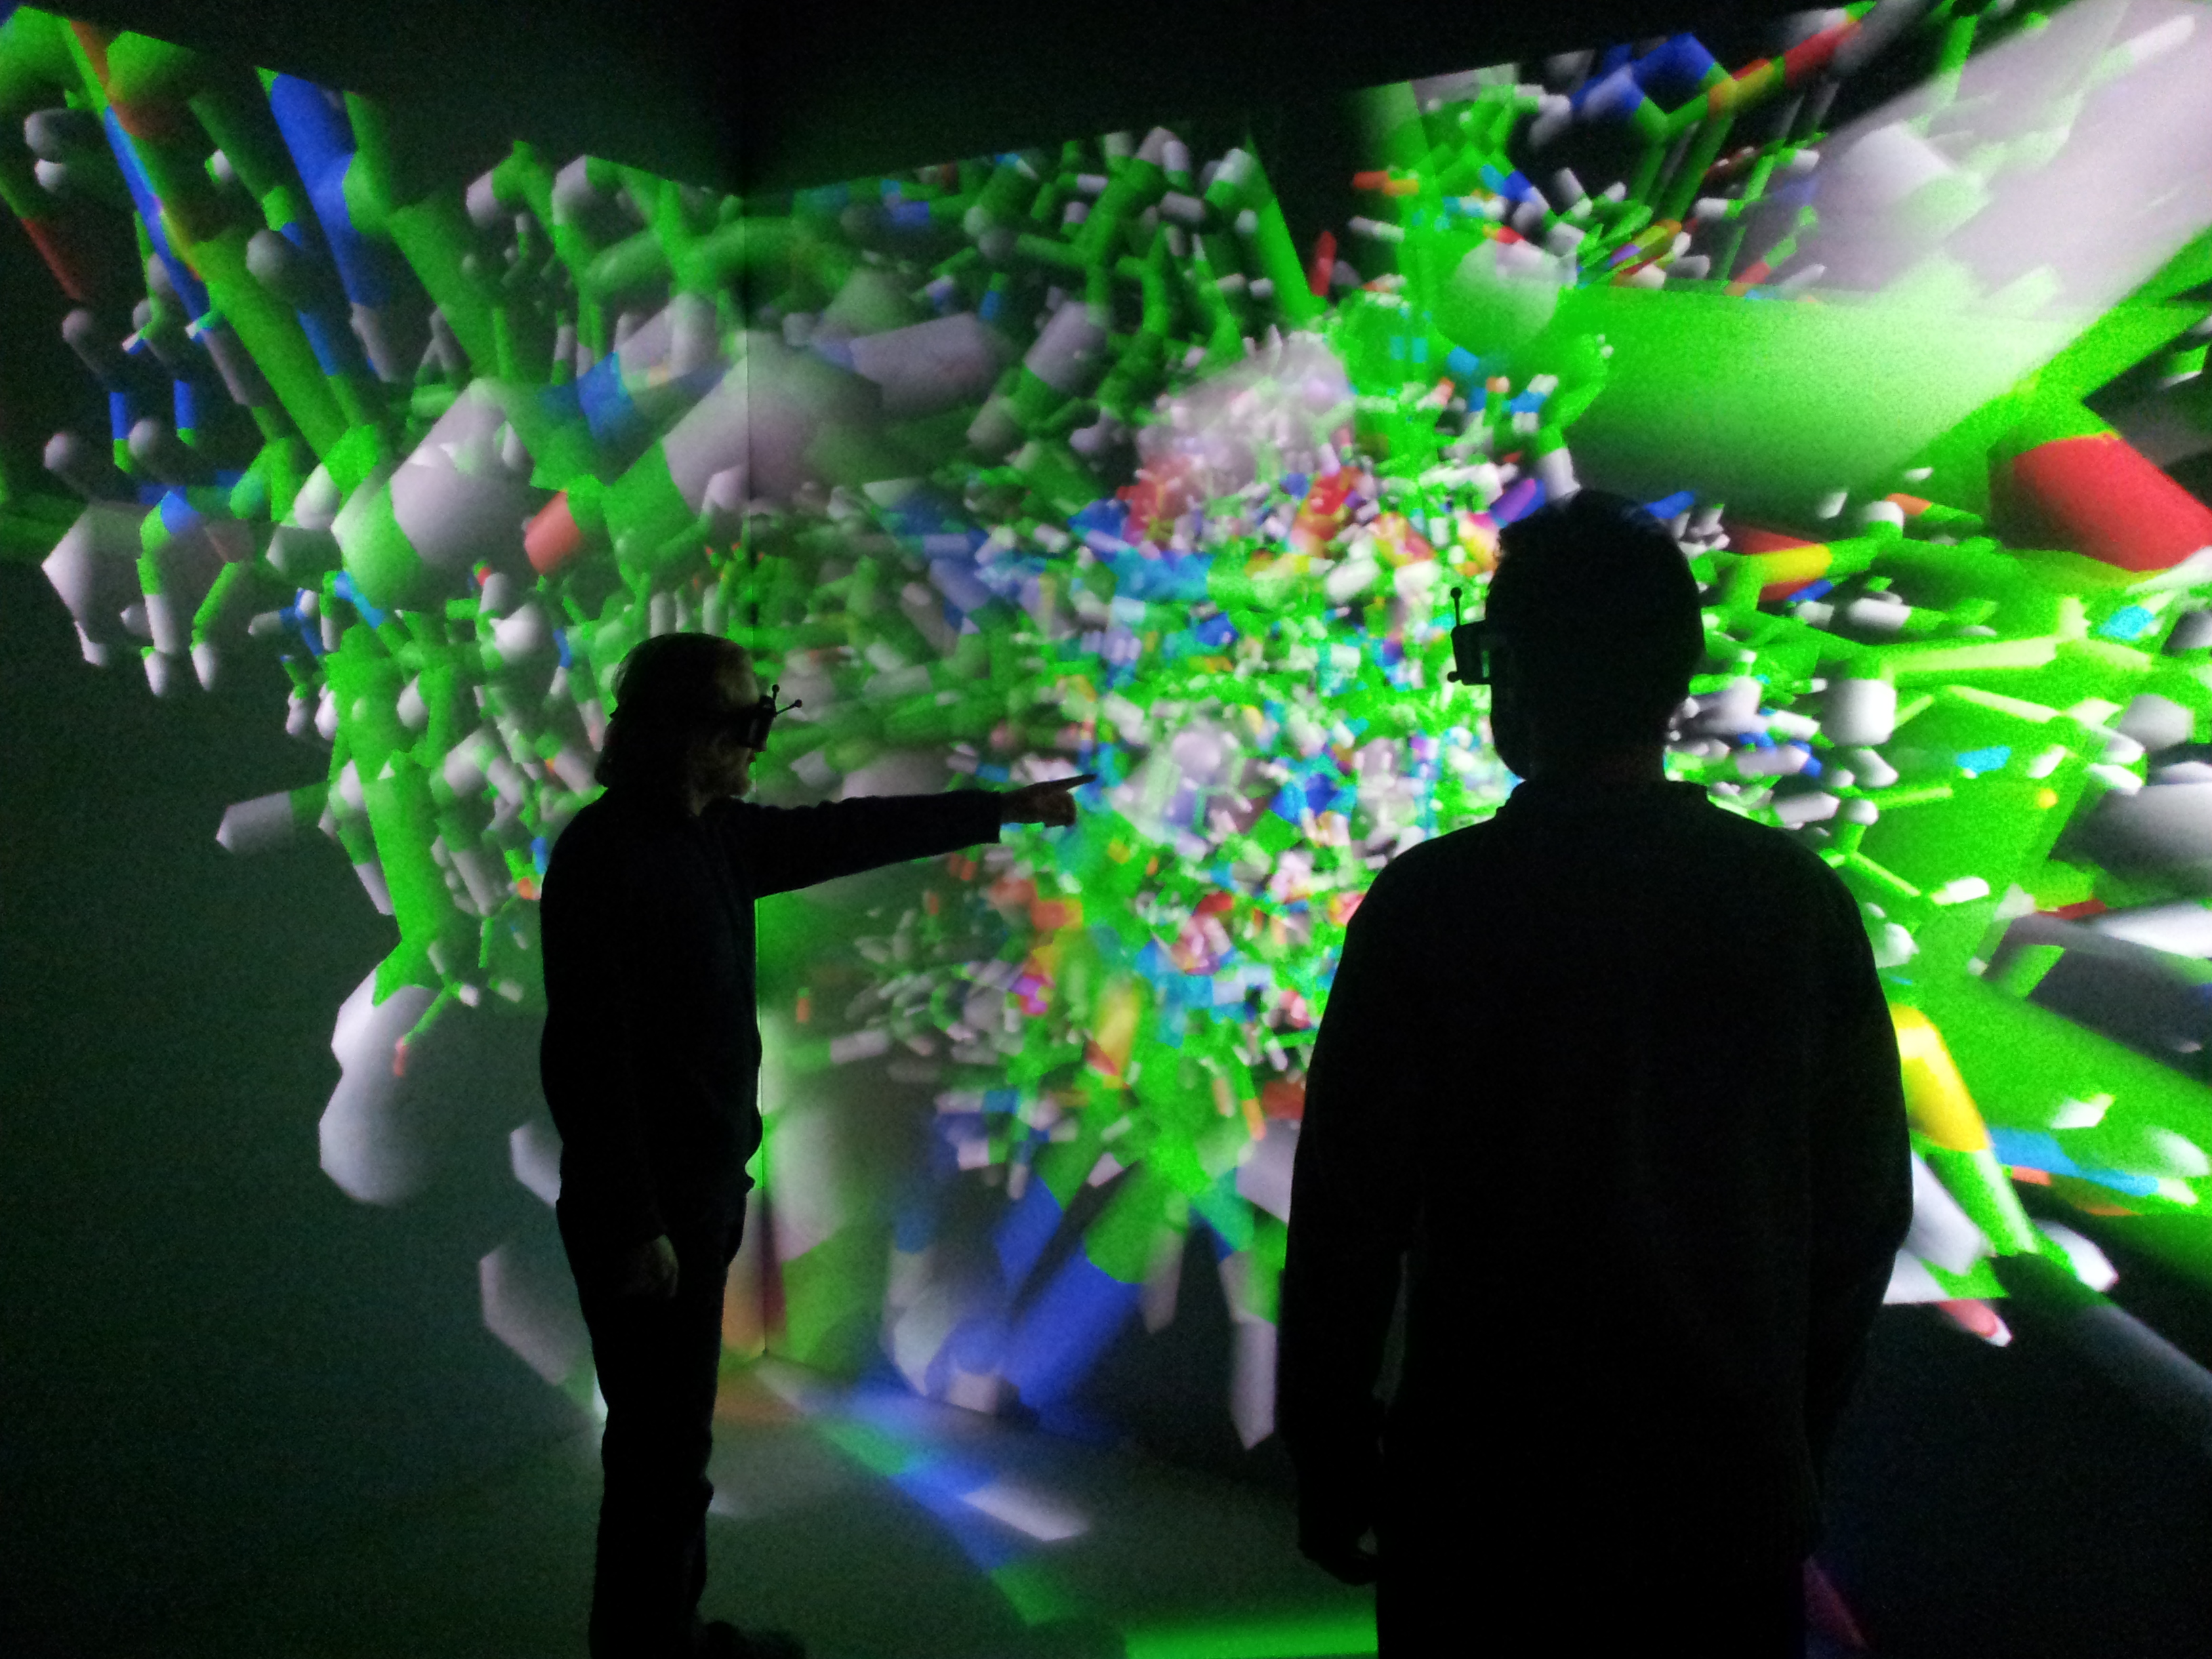
\includegraphics[width=.75\linewidth]{./figures/ch5/multi_collaboratif}}
    \caption{{\it Photo prise dans EVE, système CAVE du LIMSI/CNRS pendant une session de travail collaborative sur Moliscope.}}
  \label{Fig:multi_collaboratif}
  \hspace{0.3cm}
\end{figure}

En plus des interactions directes de commande vocale comme support des actions utilisateurs, nous avons ajouté notre moteur d'interprétation de commandes vocales vers des commandes logicielles. Notre moteur est relié à PyMol afin de donner la possibilité à l'utilisateur d'effectuer plusieurs actions pré-définies de façon simple et adaptée aux environnements immersifs.
PyMol est la partie frontale de notre application, elle est reliée indirectement à un module de gestion générique qui s'occupe de recevoir et d'émettre les informations et les événements entre l'espace de visualisation et l'espace d'analyse. Ce module est aussi construit de façon à pouvoir être relié à n'importe quel logiciel de visualisation. Il est donc indépendant de PyMol et transmet les événements liés à la visualisation à un moteur spécifique qui va s'occuper de transmettre des commandes logicielles en commandes PyMol dont la syntaxe est bien définie. PyMol pourrait donc être remplacé par un autre logiciel de visualisation moyennant une simple modification du moteur de commandes afin de l'adapter aux commandes spécifiques du logiciel utilisé.

\subsection{Visualisation des résultats d'analyses 2d}

Afin de visualiser les différents graphiques résultant des analyses effectuées \textit{a priori} ou \textit{a posteriori} de la session de travail, nous avons mis en place une interface web de visualisation/interaction avec ces graphiques. Nous souhaitions garantir une utilisation générique et indépendante du type de dispositif d'interaction. Pour ce faire, nous nous appuyons sur une librairie JavaScript de création de graphiques au sein de pages HTML appelée d3js \footnote{\url{http://d3js.org/}}. Cette librairie possède plusieurs outils de chargement de données via différentes sources, sous forme de fichiers ou à travers des flux de données. D3js permet de mettre en place des graphiques de façon relativement simple mais extrêmement paramétrables dans leur apparence ainsi que leur nature. S'appuyant sur JavaScript, elle est directement intégrée dans le code HTML d'une page web et accessible à travers toutes les plateformes permettant de visualiser du contenu HTML.

Nous utilisons un serveur web basé sur une librairie python, Flask, afin de mettre en place notre environnement web. Plusieurs extensions existent dont Flask-SocketIO qui permet aux applications Flask d'accéder à une communication bi-directionnelle et de faible latence entre le serveur et le client web. Côté client, la librairie JavaScript SocketIO est suffisante pour pouvoir envoyer et recevoir des messages vers ou depuis le serveur web Flask. Une connexion permanente peut ainsi être mise en place entre le client et le serveur (voir Figure \ref{Fig:platform_architecture}).

La plupart des événements d'interaction déclenchés par l'utilisateur au sein de la page HTML et des graphiques d3js peuvent ainsi être répercutés directement au serveur web. Suivant la nature des événements, le serveur renvoie ensuite les informations aux modules concernés.
L'espace de visualisation des résultats d'analyses est divisé en niveaux hiérarchiques structuraux qui correspondent à ceux référencés dans l'ontologie : \textit{Model} / \textit{Chain} / \textit{Residue} / \textit{Atom}. Les graphiques dessinés dans chaque niveau correspondent à des individus du niveau hiérarchique représenté. Afin de garder une cohérence entre les graphiques représentés, chaque sélection effectuée dans un graphique entraîne une mise à jour des graphiques présents dans les niveaux hiérarchiques inférieurs. Cette mise à jour se fait grâce à une requête émanant du script JS relayée ensuite au module de gestion RDF qui lancera une requête SPARQL pour les propriétés affichées dans les graphes mis à jour mais seulement pour les individus sélectionnés par l'utilisateur.

\begin{figure}
  \centering
  {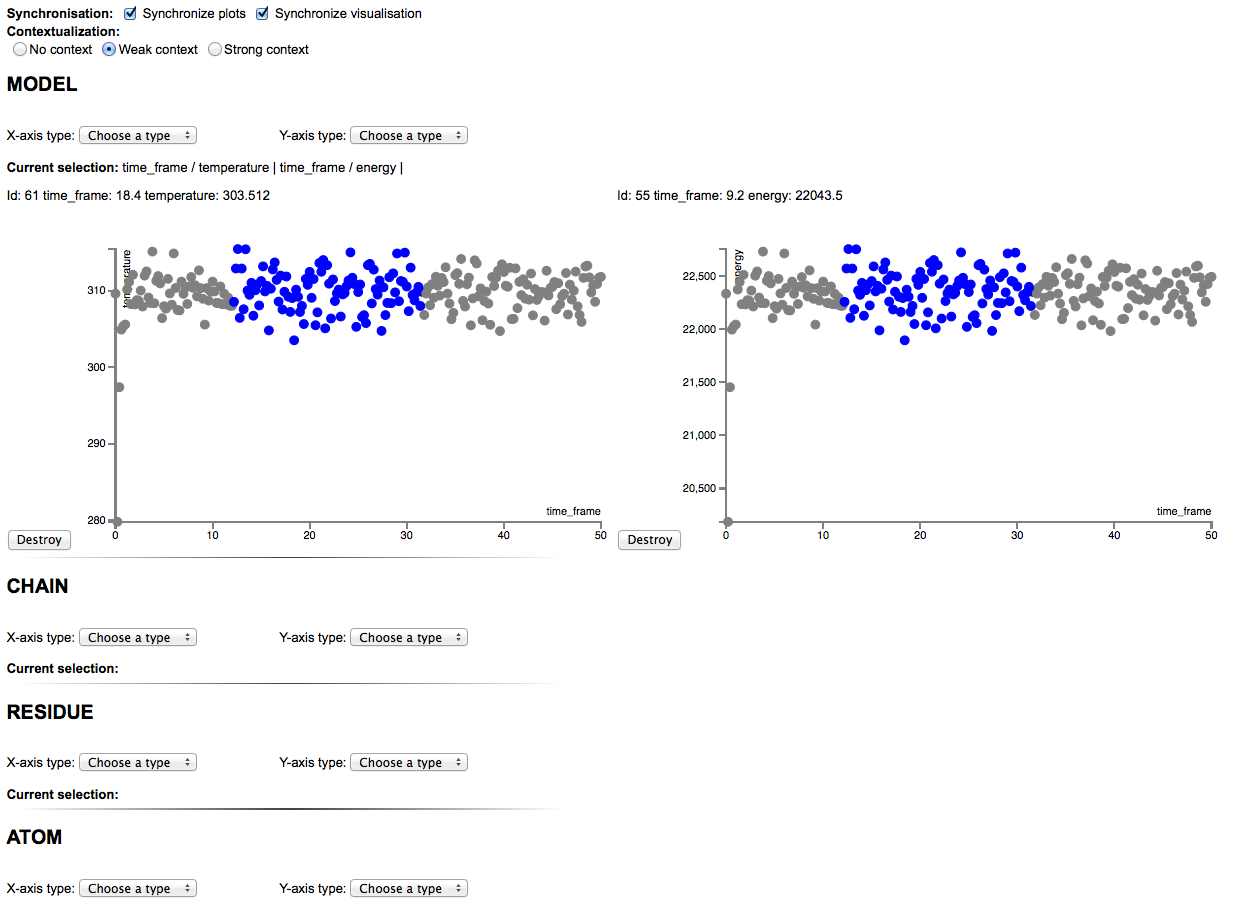
\includegraphics[width=1.0\linewidth]{./figures/ch5/2d_interface}}
    \caption{{\it Interface web 2d permettant la mise en place des graphes d'analyse sur les donnée de la base RDF.}}
  \label{Fig:multi_collaboratif}
  \hspace{0.3cm}
\end{figure}

\subsection{Analyses semi-automatiques}

Bien que la majorité des données soient présentes au sein de la base de données créée par l'utilisateur, une session de travail habituelle requiert souvent des données résultantes de calculs post-simulation et donc absentes de la base de données de départ. Ces calculs sont habituellement gérés au sein de scripts, liés ou non aux outils de simulation, et exécutés en dehors de la boucle de visualisation suite à l'observation de phénomènes particuliers lors de l'exploration des structures de la simulation ou suite à d'autres analyses déjà effectuées auparavant. Afin de ne pas surcharger la base de données et laisser l'utilisateur maître des analyses qu'il veut effectuer, nous avons profité de notre connaissance métier pour mettre en place la possibilité de lancer certaines analyses semi-automatisées pendant la session de travail. 

La force du langage de requête SPARQL est qu'il permet, en plus d'interroger une base de données, de modifier ces données, les supprimer ou en ajouter. Nous utilisons la possibilité d'ajouter des données pour permettre à l'expert d'alimenter la base de données avec des résultats d'analyses lancées pendant sa session de travail. Une liste d'analyses a été construite et chacune des analyses proposées possède sa définition ontologique. Cette définition nous permet de connaître le type de données utilisé en entrée de l'analyse et le type de données en sortie. Ainsi, suivant l'analyse désirée, la plateforme proposera un choix filtré d'individus à sélectionner, correspondant au type de donnée attendu. De la même manière, les valeurs générées en sortie de l'analyse sont automatiquement introduites dans la base de données en respectant leur définition ontologique.

% Ces analyses semi-automatisées se basent essentiellement sur les analyses utilisées usuellement par les experts du métier. Au-delà de la simple proposition d'une liste d'analyses pouvant être lancées à la volée, la connaissance du système étudié grâce à sa base de données RDF associée nous permet de proposer, pour plusieurs analyses, des données d'entrée filtrées et identifiées sur lesquelles appliquer les analyses désirées. 

L'outil \textit{Distance} nécessite par exemple deux individus de même niveau hiérarchique structural ainsi qu'une sélection d'individus de niveau hiérarchique supérieur au sein desquels seront calculés ces distances. 

Il est possible de classer ces analyses en deux catégories : Les analyses simples regroupent les analyses générant une valeur pouvant être ajoutée directement aux propriétés des individus concernés. Parmi celles-ci nous pouvons citer l'accessibilité au solvant, l'hydrophobicité, l'énergie, etc. 
Les analyses complexes sont le résultat d'une propriété décrivant un rapport entre deux individus et nécessitant donc la connaissance de ces individus pour être pertinentes. Nous pouvons citer parmi les analyses complexes reliant deux individus : la distance entre deux atomes, le RMSD entre deux ensembles d'individus, l'angle entre deux chaînes, etc.

Alors que les analyses simples ajoutent simplement à un individu une propriété et la valeur associée, les analyses complexes doivent elles créer une instance particulière d'un des concepts \textit{Analyse} de l'ontologie qui regroupera les informations nécessaires à sa compréhension. 

Le concept \textit{Distance} (de type \textit{Analyse}) de l'ontologie permettra par exemple de stocker toute distance calculée entre deux individus pour une sélection de structures parentes définies. La valeur de la distance, l'URI des deux individus impliqués ainsi que l'ensemble des structures au sein desquelles le calcul s'est effectué seront des propriétés d'une instance \textit{Distance} et seront accessibles seulement à travers cette instance. 

Cela ne complexifie donc pas seulement le stockage mais également l'accès aux informations puisque les valeurs d'analyses complexes ne sont, au contraire des analyses simples, plus directement associées aux individus concernés mais à travers un concept \textit{Analyse} intermédiaire. Il fut donc nécessaire d'adapter les requêtes SPARQL utilisées pour la génération des graphes afin de prendre en compte cette complexité. La différence entre une requête SPARQL accédant aux valeurs d'une analyse simple et la requête SPARQL permettant d'accéder à celles d'une analyse complexe est illustrée dans le Listing \ref{sparql_simple_vs_complexe}.

\begin{lstlisting}[language=XML, caption=Deux requêtes SPARQL : 1. Accès à la température d'un modèle 2. Accès à la distance entre deux résidus, label=sparql_simple_vs_complexe]
SELECT DISTINCT ?temp WHERE {my:MODEL_161 my:temperature ?temp}

SELECT DISTINCT ?distance WHERE {?indiv rdf:type my:Distance . ?indiv 
  my:objectA my:RES_3622 . ?indiv my:objectB my:RES_3626 . ?indiv 
  my:distance ?distance}
\end{lstlisting}

\subsection{Synchronisation}

La nature hétérogène des modules de notre application nous empêche d'adopter une communication directe entre les différentes instances Python créées par les différents modules. La synchronisation entre l'espace visuel et l'espace d'analyses, représenté respectivement par PyMol et le serveur web Flask, se fait au travers de communication entre leurs modules de gestion respectifs. Cette communication s'appuie sur des messages OSC envoyées par les modules à chaque événement déclenché dans un des espaces de travail. Chacun des modules est ainsi associé à un serveur OSC opérant en arrière-plan dans un sous-processus et surveillant tout message arrivant sur le port qui lui est dédié. Nous utilisons la librairie Python pyliblo \footnote{\url{http://das.nasophon.de/pyliblo/}} qui est une interface Python pour liblo \footnote{\url{http://liblo.sourceforge.net/}}, une implémentation du protocole \textit{Open Sound Control} (OSC). OSC est un format de transmission de données conçu pour être utilisé en temps réel. Pyliblo, en plus de permettre la création d'un serveur OSC, fournit également les fonctions nécessaires pour envoyer un message. Ces messages sont envoyés localement sur un port ouvert référencé par la machine qu'un serveur OSC <<surveille>> afin de détecter tout message entrant.

Les communications constantes entre les modules à travers les ports de nos serveurs OSC permettent donc d'assurer une synchronisation des actions utilisateurs dans chacun des espaces de travail. Les actions identifiées comme synchronisables sont effectuées en coordination entre les espaces.

A chaque création de graphique dans l'espace de visualisation, l'information de création est envoyée afin de créer un objet \textit{Selection} qui regroupera les informations de sélection effectuées au sein du graphique correspondant. Cet objet est référencé au sein de l'ontologie et contient : le niveau hiérarchique structural des individus, les individus sélectionnés dans le graphique, la représentation géométrique associée et le rendu visuel appliqué (couleur et transparence). Ce stockage permet de sauvegarder l'état de la visualisation à tout moment et de la corréler aux analyses présentées au sein de l'espace d'analyse. De plus, un découpage des graphiques en objet \textit{Selection} permet à l'utilisateur de choisir quels groupes de sélection il désire afficher ou cacher au sein de l'espace de visualisation. Il est donc possible de superposer les rendus visuels de chaque graphique ou d'une partie seulement suivant la volonté de l'utilisateur. Ces objets \textit{Selection} sont mis à jour à chaque interaction de l'utilisateur dans le graphique correspondant afin de refléter les individus sélectionnés. La possibilité de sauvegarder l'état de visualisation et des analyses présentes ainsi que des individus sélectionnées permet naturellement de charger un état précis d'une session de travail. Ce détail est particulièrement utile à la fin d'une longue session de travail ayant abouti à un rendu visuel satisfaisant.


\subsection{Exemple}

Dans le scénario choisi, le premier événement pris en compte au sein de l'application est le choix de l'utilisateur quant aux analyses qu'il désire afficher. Ce choix lancera une première paramétrisation de l'espace d'analyse qui pourra ainsi se connecter à l'espace de visualisation. 
Il est cependant possible de démarrer une session de travail par une exploration de la trajectoire étudiée mais cette exploration ne déclenchera pas d'événements dans l'espace visuel, ce dernier n'étant pas paramétré.

Le choix des analyses se déroule sur la page HTML et va interroger la base de données RDF afin d'identifier les propriétés pour lesquelles une valeur littérale existe pour le groupe structurel choisi par l'utilisateur. 
Ces valeurs littérales peuvent provenir de données structurales générées par la simulation moléculaire ou bien d'analyses post-simulations intégrées au sein de la base de données. 
Toutes les propriétés possédant une valeur littérale sont affichées dans deux colonnes, la première permet de choisir la propriété à afficher sur l'axe des abscisses, la seconde désigne la propriété qui sera affiché sur l'axe des ordonnées. 
L'utilisateur a la possibilité de générer plusieurs combinaisons de propriétés à afficher sous forme de graphes. 

Quand le choix est terminé, des requêtes SPARQL sont envoyées à la base de données pour récupérer les valeurs des propriétés choisies. Ces données sont ensuite mises sous forme de graphes et structurées grâce à d3js.

Lorsque les graphes sont générés, l'utilisateur a la possibilité d'interagir avec eux de différentes manières : 
\begin{itemize}
  \item Il peut sélectionner un point unique afin d'obtenir un ensemble d'informations provenant de la base de données et liés à l'individu désigné.
  \item Il est possible de sélectionner un ensemble de points dans un des graphes et afficher un cadre d'information rassemblant plusieurs statistiques sur l'ensemble des propriétés des individus ainsi sélectionnés (moyenne, écart-type, pourcentages, etc.).
  \item Il est également possible de synchroniser la sélection d'un groupe de points afin de mettre en évidence les individus concernés dans l'ensemble des graphes de la page.
\end{itemize}

Toute sélection au sein d'un ou plusieurs graphes de la page déclenche un événement transmis depuis le client web jusqu'au module de gestion 3d entraînant une adaptation de la visualisation pour mettre en avant le ou les individu(s) ayant été sélectionnés. Il est aussi possible d'obtenir, sous forme de fenêtre indépendante, un résumé des informations disponibles sur le ou les individus. Dans le cas d'un individu unique, une liste de ses propriétés et de leurs valeurs sera affichée alors que pour plusieurs individus, une moyenne effectuée sur les valeurs de leurs propriétés remplacera les valeurs brutes.
Chaque sélection réduit donc le focus de l'utilisateur à un sous-ensemble d'individus, à la fois dans l'espace d'analyses mais également de façon synchrone dans l'espace de visualisation. Il est possible d'adapter ce focus suivant les besoins de l'utilisateur en modifiant le niveau de contexte dans lequel il désire que sa sélection apparaisse. Trois niveaux de contextualisation sont possibles :
\begin{itemize}
  \item Aucun contexte - La sélection d'individu(s) entraîne la visualisation unique de ces individus dans l'espace de visualisation et d'analyse et donc cache tout individu n'étant pas sélectionné
  \item Contexte faible - La sélection d'individu(s) met en avant ces individus dans les espaces de travail et réduit la perception des autres individus du jeu de données (couleur grise, transparence, rendu visuel simplifié, etc.)
  \item Contexte fort - La sélection d'individu(s) n'est perçu qu'à travers une mise en avant simple de ces individus dans les espaces de travail. Tout autre individu apparaîtra également avec des paramètres visuels proches des individus sélectionnés.
\end{itemize}

Ces différents niveaux permettent soit de mettre en évidence les différences entre la sélection et le reste du jeu de données, soit de mettre en place un environnement de travail épuré sur une sélection d’intérêt pour l'utilisateur. Ces niveaux s'appliquent à la fois pour la partie visuelle et analytique via des systèmes de rendus visuels propres à chaque espace.

Lorsque une sous-sélection d'individus est effectuée, l'utilisateur a toute liberté pour l'explorer dans l'espace de visualisation. Si, lors de son exploration, l'utilisateur désire sélectionner un sous-groupe plus précis au sein des individus affichés, il possède deux manières de le faire : soit par une sélection directe via un dispositif d'interaction, soit par commande vocale en verbalisant le sous-groupe d’intérêt via la commande \textit{Select}.

Au-delà du changement visuel induit par la sélection dans l'espace de visualisation, ce changement va également produire un rafraîchissement de l'affichage de l'espace d'analyses, de la même manière que la précédente sélection effectuée dans l'espace d'analyses induisait une synchronisation dans l'espace de visualisation. Cependant, pour que la synchronisation ait lieu, il est nécessaire qu'au moins un graphe corresponde au niveau hiérarchique structural des individus de la sélection. Si ce n'est pas le cas, la sélection n'aura pas d'effet. Sinon, les individus seront mis en avant dans les graphes concernés. Il est cependant aussi possible, malgré la présence de graphes du bon niveau hiérarchique structural, d'activer un mode asynchrone. Dans ce mode asynchrone, aucune action effectué dans chacun des espaces n'aura d'influence sur le second espace. La synchronisation pourra se réactiver à tout moment, aux conditions exposées précédemment, lorsque les niveaux structurels des deux espaces seront identiques.


\subsection{Évaluation par la méthode HTA}

Nous avons repris la méthode HTA introduite dans la section \ref{hta_eval} afin d'évaluer les apports de nos développements pour une tâche experte identifiée et commune en biologie structurale. De la même manière que pour l'évaluation de nos paradigmes de navigation, l'évaluation au moyen de méthodes systématiques d'une plateforme dont les développements se sont basés autour de tâche experte, nous semblait dénué de sens.

Grâce à l'approche hiérarchique HTA, nous comparerons donc deux conditions de travail différentes, la première sera une utilisation classique d'un logiciel de visualisation moléculaire et d'un terminal permettant l'exploration de fichiers d'analyses. Nous ferons dans ces conditions l'hypothèse que l'ensemble des valeurs d'analyse nécessaires ont été obtenues.
La seconde condition se basera sur l'utilisation de notre programme, combinant l'utilisation d'un logiciel de visualisation moléculaire, éventuellement immersif et en interaction directe, et d'une interface web regroupant le traitement automatique des analyse en graphiques.
\\
\\
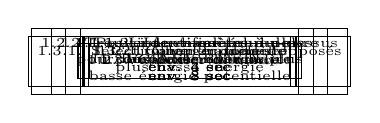
\begin{tikzpicture}
\tikzset{grow'=right,level distance=120pt}
\tikzset{execute at begin node=\strut}
\tikzset{every tree node/.style={anchor=base west}}
\Tree 
 [.\node[draw, font=\tiny, align=center]{1. Trouver le diamètre du pore\\ pour le modèle avec la plus\\basse énergie potentielle};
    [.\node[draw, font=\tiny, align=center]{1.1. Trouver modèle de\\ plus basse énergie} ;
        [.\node[draw, font=\tiny, align=center]{1.1.1. Lister modèles à plus\\ de 4A de RMSD \\ env. 8 sec}; ]
        [.\node[draw, font=\tiny, align=center](start){1.1.2. Identifier celui de \\plus basse énergie\\env. 8 sec}; ] ]
    [.\node[draw, font=\tiny, align=center]{1.2. Visualiser le modèle} ;
        [.\node[draw, font=\tiny, align=center]{1.2.1. Charger modèle \\env. 3 sec}; ]
        [.\node[draw, font=\tiny, align=center]{1.2.2. Positionner caméra au-dessus\\ du complexe moléculaire \\env. 2 sec}; ] ]
    [.\node[draw, font=\tiny, align=center]{1.3. Calculer distance};
      [.\node[draw, font=\tiny, align=center]{1.3.1. Sélectionner 2 atomes opposés \\env. 4 sec}; ]
      [.\node[draw, font=\tiny, align=center]{1.3.2. Calculer distance \\env. 4 sec}; ] ] 
    ] 
    \\           
\end{tikzpicture}
\\
\\
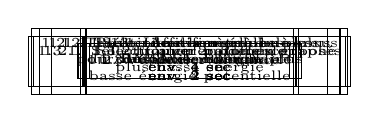
\begin{tikzpicture}
\tikzset{grow'=right,level distance=120pt}
\tikzset{execute at begin node=\strut}
\tikzset{every tree node/.style={anchor=base west}}
\Tree 
 [.\node[draw, font=\tiny, align=center]{1. Trouver le diamètre du pore\\ pour le modèle avec la plus\\basse énergie potentielle};
    [.\node[draw, font=\tiny, align=center]{1.1. Trouver modèle de\\ plus basse énergie} ;
        [.\node[draw, font=\tiny, align=center]{1.1.1. Afficher graphes \\RMSD + énergie \\ env. 4 sec}; ]
        [.\node[draw, font=\tiny, align=center]{1.1.2. Sélectionner modèles à plus\\ de 4A de RMSD \\ env. 2 sec}; ]
        [.\node[draw, font=\tiny, align=center](start){1.1.3. Identifier celui de \\plus basse énergie\\env. 2 sec}; ] ]
    [.\node[draw, font=\tiny, align=center]{1.2. Visualiser le modèle} ;
        [.\node[draw, font=\tiny, align=center]{1.2.1. Sélectionner point du graphe \\env. 1 sec}; ]
        [.\node[draw, font=\tiny, align=center]{1.2.2. Positionner caméra au-dessus\\ du complexe moléculaire \\env. 2 sec}; ] ]
    [.\node[draw, font=\tiny, align=center]{1.3. Calculer distance};
      [.\node[draw, font=\tiny, align=center]{1.3.1. Sélectionner 2 atomes opposés \\env. 4 sec}; ]
      [.\node[draw, font=\tiny, align=center]{1.3.2. Calculer distance \\env. 4 sec}; ] ] 
    ] 
    \\           
\end{tikzpicture}
\\


Le scénario de tâche que nous avons choisi peut être divisé en trois étapes distinctes. Il nécessite une première étape de traitement des données d'analyse où l'on cherchera le modèle de plus basse énergie parmi les modèles distants de plus de 4\r{A} de RMSD du modèle de référence. Lorsque le modèle concerné est identifié, il convient de le visualiser de façon appropriée le complexe moléculaire de façon à voir le pore et pouvoir sélectionner ses extrémités. La troisième étape consiste finalement à calculer la distance entre deux atomes de part et d'autre du pore.
On retrouve un temps d'exécution significativement inférieur lors de l'utilisation de notre programme (19 s) comparé à une utilisation standard des outils d'analyse et de visualisation (29 s). La première étape d'analyse est l'étape où la différence est la plus importante. Cette différence s'explique par l'utilisation de graphes interactifs pour visualiser les valeurs de RMSD et d'énergie pour l'ensemble des modèles. Cet outils nous permet de mettre en avant par un simple rectangle de sélection l'ensemble des modèles à plus de 4\r{A} du modèle de référence. L'identification du modèle de plus basse énergie au sein des modèles mis en avant consiste ensuite en une simple analyse visuelle du graphe d'énergie.
A l'opposé, l'utilisation d'outils en ligne de commandes est beaucoup plus fastidieuse car nécessite un traitement visuel plus complexe. Il est en effet beaucoup plus aisé de trouver une valeur minimale au sein d'un nuage de point qu'au sein d'un fichier texte simple. L'étape de chargement du modèle au sein du logiciel de visualisation est également plus simple puisque notre application permet d'interpréter une sélection du modèle concerné dans un graphique directement dans le logiciel de visualisation grâce à un filtre affichant uniquement le modèle concerné.

Un second scénario a été étudié, comparant les mêmes conditions que précédemment.
\\
\\
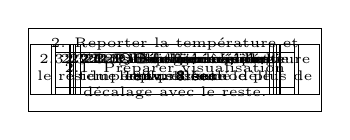
\begin{tikzpicture}
\tikzset{grow'=right,level distance=120pt}
\tikzset{execute at begin node=\strut}
\tikzset{every tree node/.style={anchor=base west}}
\Tree 
 [.\node[draw, font=\tiny, align=center]{2. Reporter la température et\\ l'énergie du modèle dont\\ le résidue 182 présente le plus de\\ décalage avec le reste.};
    [.\node[draw, font=\tiny, align=center]{2.1. Préparer visualisation} ;
        [.\node[draw, font=\tiny, align=center]{2.1.1. Charger modèles \\ env. 4 sec}; ]
        [.\node[draw, font=\tiny, align=center](start){2.1.2. Souligné résidu\\env. 2 sec}; ]
        [.\node[draw, font=\tiny, align=center](start){2.1.3. Déplacer caméra\\env. 3 sec}; ] ]
    [.\node[draw, font=\tiny, align=center]{2.2. Identifier résidu\\ le plus décalé} ;
        [.\node[draw, font=\tiny, align=center]{2.2.1. Observation visuelle \\env. 10 sec}; ]
        [.\node[draw, font=\tiny, align=center]{2.2.2. Sélection résidu\\env. 2 sec}; ] ]
    [.\node[draw, font=\tiny, align=center]{2.3. Obtenir énergie et \\température du modèle};
      [.\node[draw, font=\tiny, align=center]{2.3.1. Parser fichier énergie \\env. 8 sec}; ]
      [.\node[draw, font=\tiny, align=center]{2.3.2. Parser fichier température \\env. 8 sec}; ] ] 
    ] 
    \\           
\end{tikzpicture}
\\
\\
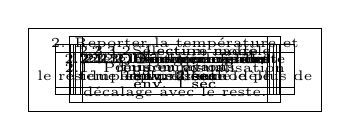
\begin{tikzpicture}
\tikzset{grow'=right,level distance=120pt}
\tikzset{execute at begin node=\strut}
\tikzset{every tree node/.style={anchor=base west}}
\Tree 
 [.\node[draw, font=\tiny, align=center]{2. Reporter la température et\\ l'énergie du modèle dont\\ le résidue 182 présente le plus de\\ décalage avec le reste.};
    [.\node[draw, font=\tiny, align=center]{2.1. Préparer visualisation} ;
        [.\node[draw, font=\tiny, align=center]{2.1.1. Charger modèles \\ env. 4 sec}; ]
        [.\node[draw, font=\tiny, align=center](start){2.1.2. Souligné résidu\\env. 2 sec}; ]
        [.\node[draw, font=\tiny, align=center](start){2.1.3. Déplacer caméra\\env. 3 sec}; ] ]
    [.\node[draw, font=\tiny, align=center]{2.2. Identifier résidu\\ le plus décalé} ;
        [.\node[draw, font=\tiny, align=center]{2.2.1. Observation visuelle \\env. 10 sec}; ]
        [.\node[draw, font=\tiny, align=center]{2.2.2. Sélection résidu\\env. 2 sec}; ] ]
    [.\node[draw, font=\tiny, align=center]{2.3. Obtenir énergie et \\température du modèle};
      [.\node[draw, font=\tiny, align=center]{2.3.1. Sélection modèle \\ mis en avant\\env. 1 sec}; ]
      [.\node[draw, font=\tiny, align=center]{2.3.2. Lecture cadre \\ d'informations \\env. 1 sec}; ] ] 
    ] 
    \\   
\end{tikzpicture}
\\

Nous nous sommes intéressés dans cette tâche au processus inverse que celui étudié précédemment. Alors que la démarche précédente était de chercher des informations d'analyses pour guider la navigation, nous sommes ici partis d'une observation faite pendant l'exploration afin d'ensuite caractériser analytiquement le phénomène.
Un nouveau découpage en trois principales étapes peut être effectué. Il comprend d'abord la préparation de l'étape de visualisation. Même si cette étape peut être partiellement automatisée au sein de notre plateforme, nous faisons l'hypothèse que les étapes de préparation sont identiques. Les temps d'exécution sont donc identiques (9 s).
La seconde étape est l'identification visuelle du résidu concerné. Cette étape ne présente pas non plus de différences entre les deux approches dont les temps sont une nouvelle fois égaux (12 s). Elle est étroitement liée au logiciel de visualisation et à l'exploration du complexe moléculaire 3d.
La dernière étape marque la plus grande différence de performance entre les deux conditions. En effet, elle concerne la prise d'informations au sein de l'espace d'analyses après identification du modèle concerné dans l'espace de visualisation. Une simple sélection du résidu mettra en avant le modèle concerné dans l'espace d'analyse au sein de notre programme et que les informations liées à cet individu seront demandées instantanément à la base de données (2 s). Dans des conditions standards, le processus de recherche d'informations passe par le traitement manuel des fichiers concernés et n'est aucunement facilité par une quelconque interaction provenant du logiciel de visualisation (16 s).

On observe à travers ces deux scénarios un avantage significatif de l'utilisation de notre programme lorsque la sélection d'un sous ensemble d'espace de travail (visualisation ou analyse) permet le filtrage des données de l'espace complémentaire. Quand ces deux espaces sont séparés, comme c'est le cas dans des conditions de travail normales, les aller-retours entre les informations sont fastidieuses et prennent un temps plus important. Notre évaluation a porté sur des tâches courtes et ponctuelles, elle peut cependant être étendue à des tâches plus complexes ou des séquences de tâches similaires où on s'attendrait à une différence de temps d'exécution encore plus importante.

\section{Résumé et conclusion}
\label{sec:ConclusionVisuAna}

Afin d'optimiser le travail autour de l'étude de structures moléculaires au sein d'un environnement immersif, nous avons développé une plateforme logicielle basée sur une communication interactive entre deux espaces indispensables en biologie structurale : un espace de visualisation et un espace d'analyses. Cette communication entre deux espaces aux caractéristiques différentes est rendue possible grâce à la représentation sémantique de l'ensemble des concepts avec lesquels l'utilisateur interagit lors d'une session de travail. Ces concepts peuvent être aussi bien scientifiques, et concernés les données manipulées et observées, que logiciels, décrivant les composants et les actions de la plateforme choisie. 

L'ontologie créée et le formalisme RDF/RDFS permettent une homogénéité des données échangées entre l'ensemble des modules de calculs (rendu visuel, analyses, simulation) puisque chaque module peut accéder aux données qu'il utilise au sein de la base de données construite autour de cette ontologie. On retrouve cette notion d'homogénéité en dehors de l'utilisation même de l'application puisque la représentation ontologique des concepts permet également d'assurer une cohérence et un modèle commun de données à respecter par les utilisateurs lors de la mise en place de nouvelles bases de données de complexes moléculaires. Ainsi, il est possible de mettre en commun certaines informations et d'enrichir les connaissances grâce à des requêtes croisées SPARQL par exemple. La communication inter-modules est la clé de voûte de notre application et l'approche passant par représentation sémantique des données favorise grandement sa mise en place. Cette approche n'a pas pour seul effet de garantir la cohérence des données échangées, elle permet aussi l'anticipation de certaines actions de l'utilisateur et donc de mettre en place des processus d'interaction directe requis dans les environnements immersifs dans lesquels nous travaillons.

Notre plateforme, malgré son architecture multi-composant impliquant un nombre important de communications, respecte les contraintes temporelles inhérentes à tout application interactive. La figure X montre les temps d'exécution des principales actions utilisateurs lors d'une session de travail. On constate qu'elles sont toutes réalisables dans un temps considéré comme interactif puisque de l'ordre de ce que l'on pourrait attendre pour une application standard.

Les bases de données sont un excellent moyen de stocker et mettre à disposition à tout instant les informations obtenues par l'utilisateur lors de ses sessions immersives de travail. Chaque nouvelle analyse met en jeu des résultats qui seront automatiquement stockés dans la base de données et réutilisables par la suite. Ceci assure une continuité dans le travail et permet de reprendre toute session à un point bien particulier. Les possibilités de partager ainsi une session de travail entre collaborateurs ou de reprendre une session de travail à l'état où elle se trouvait lors de sa dernière utilisation sont des caractéristiques que la majorité des scientifiques apprécient lors de l'utilisation de leurs outils. L'étude de l'évolution de structures moléculaires est un processus long et, comme évoqué précédemment, structuré en boucles successives, il est donc important d'être capable d'avoir un suivi stricte du travail effectué. La communication est également un enjeu majeur dans les sciences où le partage des informations entre collaborateurs et scientifiques du même milieu est primordial puisqu'elle constitue une partie des processus d'évaluation. Il est possible d'aller plus loin dans ce partage d'informations au sein de notre application en développant l'aspect collaboratif. L'une des forces de notre application repose également sur son développement autour d'une base de données construite autour d'une ontologie indépendante et déportée. Les modules au coeur de l'application n'ont aucune connaissance des logiciels ou librairies utilisés pour l'affichage 2d et 3d. Cette dissociation permet le couplage d'un nombre important de logiciels de visualisation 3d et 2d. Ce couplage passerait par un simple portage des modules de conversion des données en commandes spécifiques pour les logiciels de visualisation choisis.


